\documentclass{article}

\usepackage[tmargin=1in,bmargin=1in,lmargin=1.25in,rmargin=1.25in]{geometry}
\usepackage{graphicx}
\usepackage{hyperref}
\hypersetup{
    colorlinks=true,
    linkcolor=blue,
    filecolor=magenta,      
    urlcolor=cyan,
}
\usepackage{ragged2e}
\usepackage{soul}
\usepackage{enumitem}

\usepackage[dvipsnames]{xcolor}
\usepackage[tikz]{bclogo}

\usepackage{cite} 
\usepackage{multirow}

\usepackage{graphicx}
\usepackage{float}
\usepackage{arydshln}
\usepackage{dsfont}

\usepackage{scalerel,stackengine}

\graphicspath{{inputs/}}

\usepackage[bottom,flushmargin]{footmisc}

\usepackage{picture}
\usepackage{booktabs}
\usepackage{caption} 
\captionsetup[table]{skip=2pt}
\usepackage{dblfloatfix}
\usepackage{xcolor}
\usepackage[normalem]{ulem}
\usepackage[toc,page]{appendix}
\usepackage{footnote}
\makesavenoteenv{tabular}
\makesavenoteenv{table}

\usepackage{framed,color}
\usepackage[framemethod=tikz]{mdframed}
\usepackage{lipsum}

\usepackage{amsmath}
\usepackage{amsmath,amssymb}
\usepackage[font=small,skip=0pt]{caption}

\DeclareRobustCommand{\bbone}{\text{\usefont{U}{bbold}{m}{n}1}}
\DeclareMathOperator{\EX}{\mathbb{E}}

\usepackage{afterpage,natbib,lipsum}
\hypersetup{%
   citecolor=blue
}

\usepackage{fancyhdr}
\pagestyle{fancy}
\fancyhf{}
\lfoot{\it NBA Analytics} 
\cfoot{} 
\rfoot{\thepage}
\fancypagestyle{plain}{%  the preset of fancyhdr 
    \fancyhf{} % clear all header and footer fields
    \lfoot{{\it NBA Analytics}}
    \cfoot{} 
    \rfoot{\thepage}}
    
    
\usepackage{manfnt}
\reversemarginpar
\newcommand{\marginsymbol}{\leavevmode{\marginpar{\bcdanger}}}

\usepackage{marginnote}

\usepackage{movie15}
\usepackage{animate}

\usepackage{subcaption}
\usepackage{caption}

\newcommand\reallywidehat[1]{%
\savestack{\tmpbox}{\stretchto{%
  \scaleto{%
    \scalerel*[\widthof{\ensuremath{#1}}]{\kern-.6pt\bigwedge\kern-.6pt}%
    {\rule[-\textheight/2]{1ex}{\textheight}}%WIDTH-LIMITED BIG WEDGE
  }{\textheight}% 
}{0.5ex}}%
\stackon[1pt]{#1}{\tmpbox}%
}

\begin{document}


\title{{ \bf ReboundNet: Advanced Rebounding Metrics for NBA Basketball}}
\author{James Venzor}
\maketitle

\begin{abstract}
\noindent
With the onset of NBA player tracking data, much attention has been given to quantifying offensive and defensive metrics. This paper focuses on the often overlooked aspect of rebounding. In this paper, we leverage NBA player tracking data from the first half of the 2015--2016 NBA season to identify rebounding plays. We derive relevant features from the time of the shot attempt, and identify the expected landing spot of all shots, to train a convolutional neural network on over 33,000 historical rebounding plays. This model, which we call ReboundNet, accurately predicts the rebounder on holdout plays 49\% of the time. From these ReboundNet predictions, we produce rebounding evaluation metrics at the team and player levels.
\end{abstract}

\section{Introduction}

\noindent
An often overlooked aspect of the game of basketball is rebounding. A team that efficiently rebounds the basketball can both maximize its number of possessions and minimize its opponents possessions. In this way, rebounding indirectly contributes to a team's ability to score and also impede its opponent from scoring.
\bigbreak
\noindent
The most commonly tabulated rebound statistic for a player is {\it rebounds per game}. This metric is convenient since it can be derived from box score data, but is flawed because each game provides players with varying number of rebound opportunities. Consider that during the course of a game, one player may be present on the court for more missed shots than another player, and hence may be given more opportunities to record rebounds. The introduction of Sports VU player tracking data enabled the creation of a more robust rebounding stat called {\it rebounds per opportunity}. This improved statistic captures the rate at which a player records a rebound given an opportunity, with an opportunity defined as a player being within 3.5 ft of a rebound.
\bigbreak
\noindent
While an improvement over the rebounds per game metric, the rebounds per opportunity metric is not without its own flaws. First, it uses an arbitrary cutoff of 3.5 ft to define a rebounding opportunity. More concerning, it only considers each individual player's position relative to the eventual rebound location. In doing so, it assumes that all players within 3.5 ft of the rebound location have an equal shot at grabbing the rebound. Moreover, it assumes that all players outside of 3.5 ft of the eventual rebound location have no chance of recording a rebound. Such assumptions introduce bias into the metric by ignoring critical basketball-specific interactions that effect rebounding, such as box-outs, floor--spacing, and defensive assignments.
\bigbreak
\noindent
This paper provides a novel method for evaluating rebounding that leverages Sports VU player tracking data to create a convolutional neural network that assigns rebound probabilities to {\it all} 10 players on the court based on their relative positions and speeds at the time of a shot, and the eventual landing point of the shot if it were not touched. In this way, the neural network produced is able to learn the important interactions among all players that dictate which players are in a favorable position to record a rebound at the time of a shot attempt. These probabilities can subsequently be used for team and player rebounding evaluation.

\clearpage

\section{Methods}

\subsection{Data Collection}

\noindent
The NBA released Sports VU player tracking data from the first half of the 2015-2016 NBA season, providing data from over 600 NBA games. I obtained this Sports VU player tracking data from \href{https://github.com/sealneaward/nba-movement-data}{this github repo}. These data provide information on the 2--dimensional positioning of all players on the court, as well as the 3--dimensional positioning of the basketball, taken 25 times per second. Additionally, play-by-play data is also included, so that each play can be tagged with its shooter, rebounder, etc.

\bigbreak
\noindent
We can analyze rebounding plays from these data by focusing on the portions of the data just prior to the time of a missed shot, and through the eventual rebound. An example of such data, from a 2016 game between the Charlotte Hornets and Toronto Raptors, is animated in \textcolor{blue}{Figure} \ref{fig:ReboundExAnimation} below (open this file in Adobe Acrobat and click on the figure to play animation).

\begin{figure}[htb]
\animategraphics[width=\columnwidth]{8}{ReboundExGif2/gganim_plot}{0005}{0049}
\caption{\bf{Animation of Rebounding Play}}
\label{fig:ReboundExAnimation}
\end{figure}

\noindent
Our goal is to predict all 10 player's rebound probability for any given play. But at what point in the play do we want to make this prediction? The optimal point in time to make this prediction is at the time of the shot, since it is at precisely this time that players begin attempting to secure an eventual rebound by battling for position and judging the landing spot of the ball\footnote{To gain intuition on this point, compare the motion of all players in \textcolor{blue}{Figure} \ref{fig:ReboundExAnimation} before and after the time of the shot.}. Additionally, we need to consider the landing spot in our analysis, as where the ball bounces is a critical factor to who eventually rebounds the basketball (referencing at the animation in \textcolor{blue}{Figure} \ref{fig:ReboundExAnimation}, it is clear that Luis Scola benefited from the bounce of the ball, while Jonas Valanciunas was hindered by it). 

\bigbreak
\noindent
Keeping this in mind, the above animation contains a significant amount of superfluous data to our aim. However, it also contains all of the information we need to determine the time of the shot and the shot's eventual landing spot. This information can be derived from the animation as follows:
\begin{enumerate}
	\item{\underline{{\bf Time of Shot}}}
	\newline
         \noindent
	 Ideally, we could define the time of shot as the exact time the ball left the shooters hand. Unfortunately, this is not directly available through the player tracking data. Rather, we approximate this by defining the time in which the basketball had the largest acceleration prior to entering a shot arc as the time of a shot.
	\item{\underline{{\bf Eventual Landing Spot of Shot}}}
	\newline
         \noindent
         The eventual landing spot of the ball was obtained by applying physics\footnote{Specifically, we solve the system of equations: 1) $z_f = z_0 + v_zt + \frac{1}{2}a_zt^2 $, 2) $x_f = x_0 + v_xt $, and 3) $y_f = y_0 + v_yt $ where $x_0, y_0, z_0, v_x, v_y, $ and $v_z$ are known from the player tracking data, and $a_z = g_z = 9.81 \frac{m}{s} $, and $(x_f, y_f)$ is the determined landing location.} to the motion of the basketball upon deflecting off of the basket (or backboard). Since we can identify when the basketball is leaving the hoop, and can pin down its positioning and velocity in 3-dimensions, we can approximate its landing point if it was not touched.
\end{enumerate}	

\bigbreak
\noindent
We can now simplify each rebounding play to a still shot image of the court at the time of the shot attempt, supplemented with  the estimated landing spot of the shot. Additionally, since we know the results of the plays in our dataset, we can also record the eventual rebounder for each play! For the play animated in \textcolor{blue}{Figure} \ref{fig:ReboundExAnimation}, this results in the image shown below in \textcolor{blue}{Figure} \ref{fig:ReboundExNoProbs}.

\begin{figure}[htb]
\centering
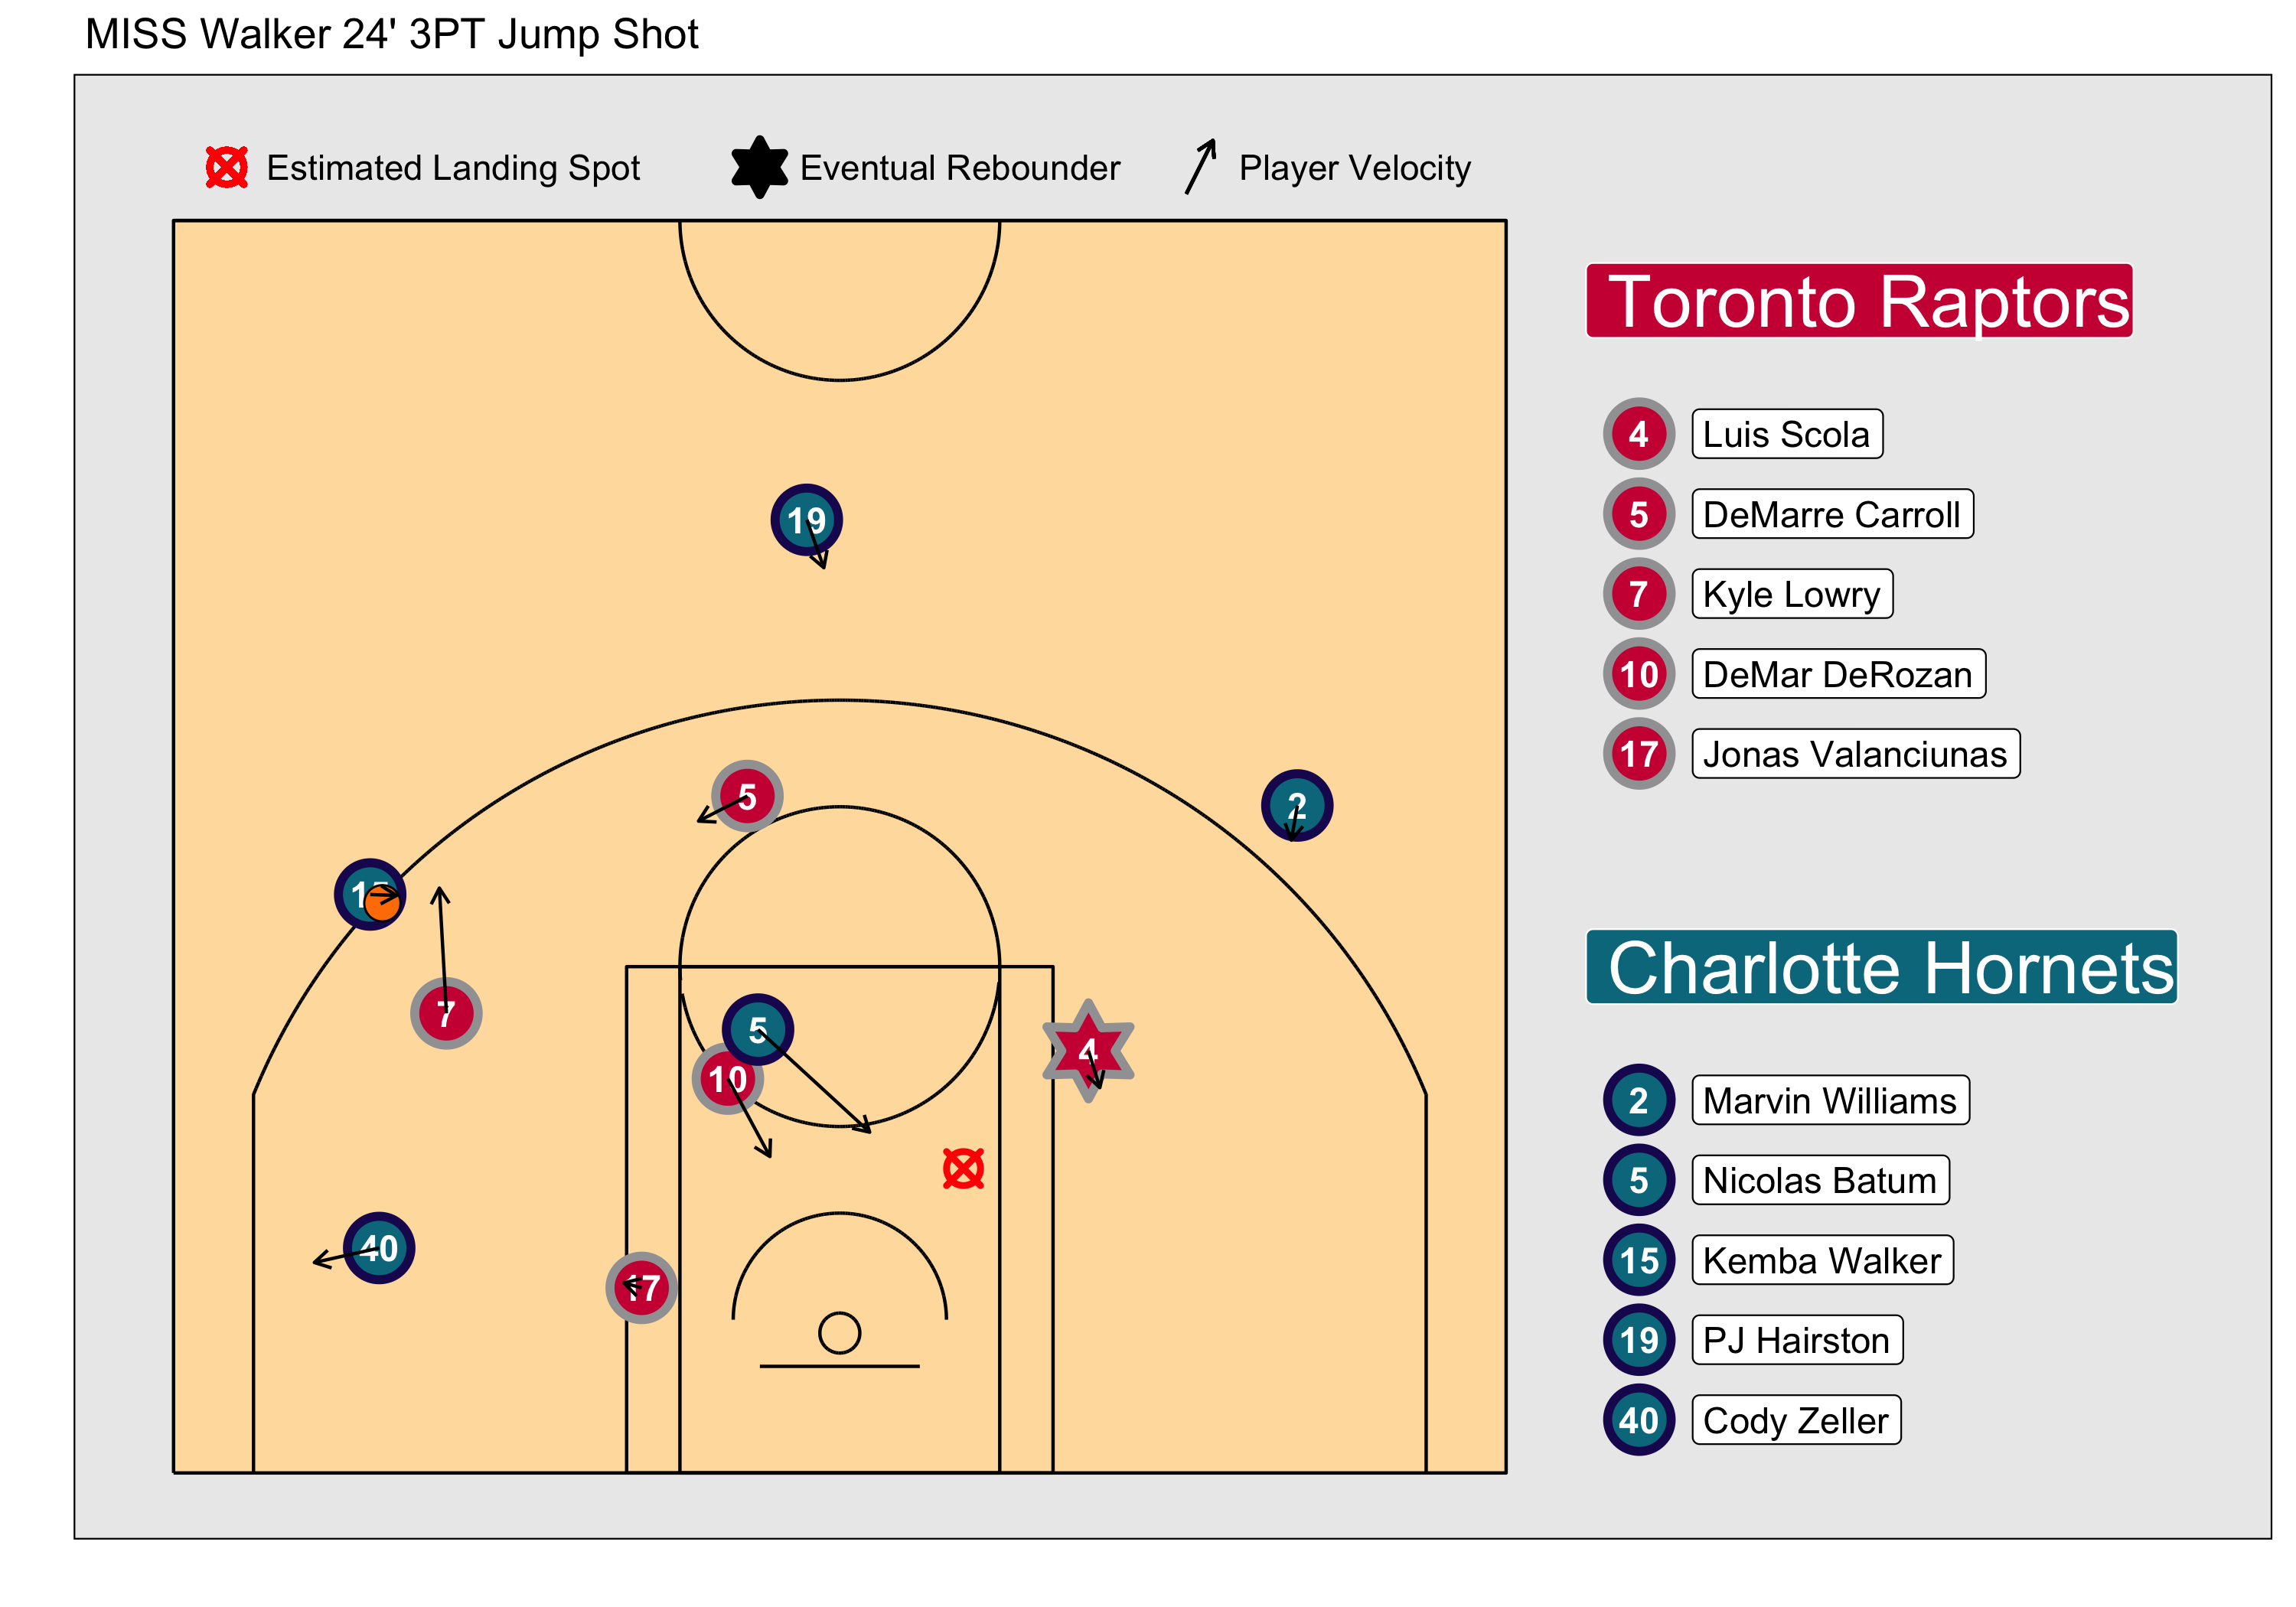
\includegraphics[width=1\columnwidth]{ReboundExNoProbs.png}
\caption{\bf{Snapshot of Rebounding Play}}
\label{fig:ReboundExNoProbs}
\end{figure}

\noindent
All rebounding plays present in the available player tracking data were analyzed in this manner. Plays with no individual rebounder\footnote{These plays are referred to as team rebounds, and commonly occur when a ball is knocked out of bounds after a missed shot.} were excluded from the analysis, as well as any blocked shots, missed dunks, beyond half--court shots, or consecutive tip shots, as these plays were deemed to be distinct in nature from that of a normal rebounding play. Additionally, shots occurring with less than 10 seconds remaining in the quarter were excluded, as there may not have been sufficient motivation to obtain a rebound if time would run out regardless. 

\noindent
After such exclusions, we were left with 33,089 rebounding plays. To check the data collected, the collective shot locations and estimated landing locations are plotted below in \textcolor{blue}{Figure} \ref{fig:QAHeatMaps} as heat maps. We see the expected behavior that shots are mainly from either behind the 3--point line, or near the basket, and the expected landing spots occur with highest frequency closest to the basket.

\begin{figure}[htb]
\centering
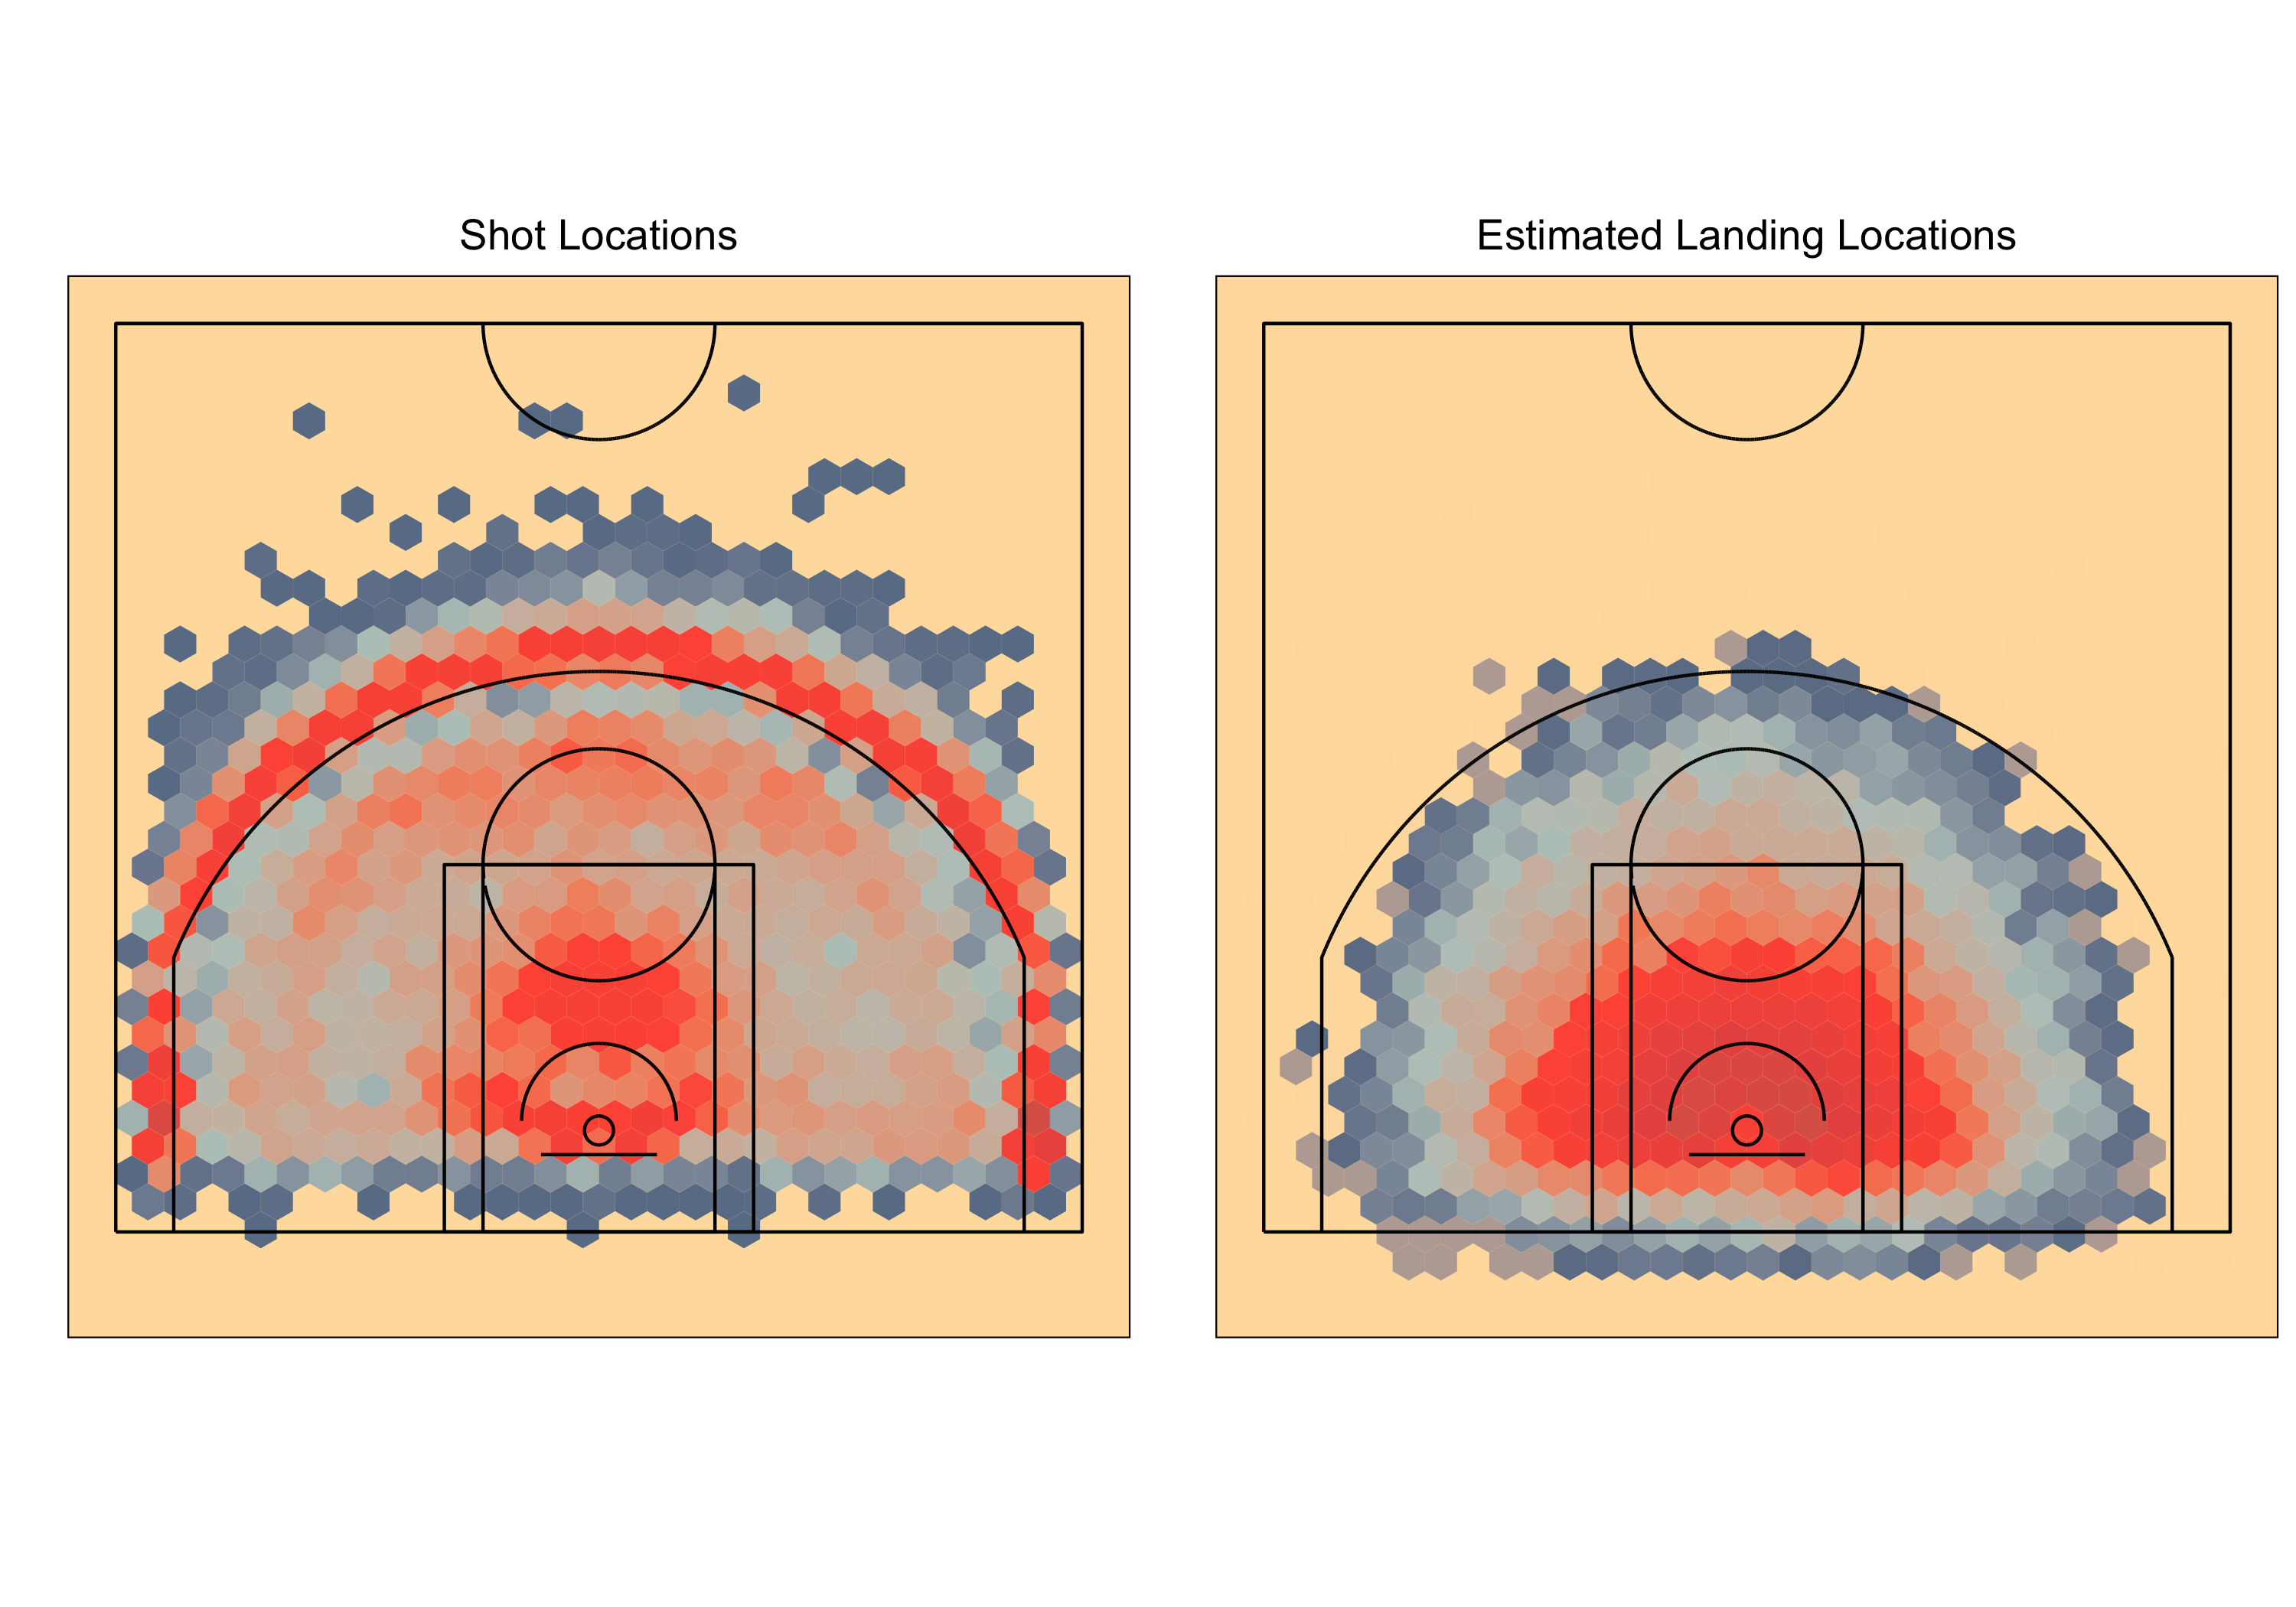
\includegraphics[width=.9\columnwidth]{EDAplots.png}
\caption{\bf{Summary of 33,089 Plays Included in Analysis}}
\label{fig:QAHeatMaps}
\end{figure}

\subsection{Model Structure}

\bigbreak
\noindent
Our goal is to predict the probability that each player on the court records a rebound at the time of a shot, given the type of information show in \textcolor{blue}{Figure} \ref{fig:ReboundExNoProbs} (except for knowledge of who got the rebound!). In order to do this, it was necessary to make some key assumptions. 

\bigbreak
\noindent
The main assumption made is that for a given rebounding opportunity, all players on the same team will attempt to obtain a rebound independently of each other. This is a realistic assumption, since players on the same team will never box each other out, and rarely impede each other's motion (this assumption breaks down for plays where a player is close to a triple double, and his teammates allow him to record a rebound he otherwise would not have obtained). However, we do not assume that pairs of opponents attempt to grab the rebound independently. Rather, we hold that due to factors such as boxouts and defensive assignments, it is necessary to allow our analysis to capture interactions between opponents. With these assumptions in mind, various features were derived in order to predict player rebound probabilities. The features that were deemed informative are summarized below.

\bigbreak
\noindent
\underline{{\bf Rebounding--Specific Features}}:
Let $X,Y$ represent the components of a 2-dimensional location on the court, and $S_{x,y}$ represent the components of a 2-dimensional velocity. Additionally, let $P$ represent the position of a player, where $P = 0, 1, $ or $2$ if a player is a guard, forward, or center respectively\footnote{This was used in place of variables such as height or weight, as these were not available from the released data.}. Finally, let $\delta = 0$ if a player is on offense and $\delta = 1$ if the player is on defense. Then, the informative features discovered were:

\bigbreak
\begin{enumerate}
\itemsep0em 
	\item{Player $X,Y$ - Opponent $X,Y$}
	\item{Player $S_{x,y}$ - Opponent $S_{x,y}$}
	\item{Player $P$ - Opponent $P$}
	\item{Player $X,Y$ - Basket $X,Y$}
	\item{Player $X,Y$ - Shot Landing $X,Y$}
	\item{Player $X,Y$ - Shooter $X,Y$}
	\item{Player $S_{x,y}$}
	\item{Player $P$}
	\item{Player $\delta$}
\end{enumerate}	

\bigbreak
\noindent
Features 1--3 above capture necessary interactions across all player/opponent combinations. For each player, we know their distance from each opponent, difference in speed from each opponent, and difference in position with opponent (for example, if it is a guard taking on a center). 

\bigbreak
\noindent
Features 4--6 give all necessary contextual information on a player's location. Specifically, we know each player's distance from the basket, shot landing spot, and shooter. Features 7--9 give non-location based information about each player, comprising of each player's velocity, position, and if that player is on offense or defense.
\bigbreak
\noindent
These features were used to form a 3-dimensional tensor to represent each play, and were fed to a neural network model, which we call ReboundNet. The simplified structure of ReboundNet is shown below. This structure (and its representation) were inspired by the winners of the 2020 NFL Big Data Bowl, whose submission is linked to \href{https://www.kaggle.com/c/nfl-big-data-bowl-2020/discussion/119400}{here}.

\begin{figure}[htb]
\centering
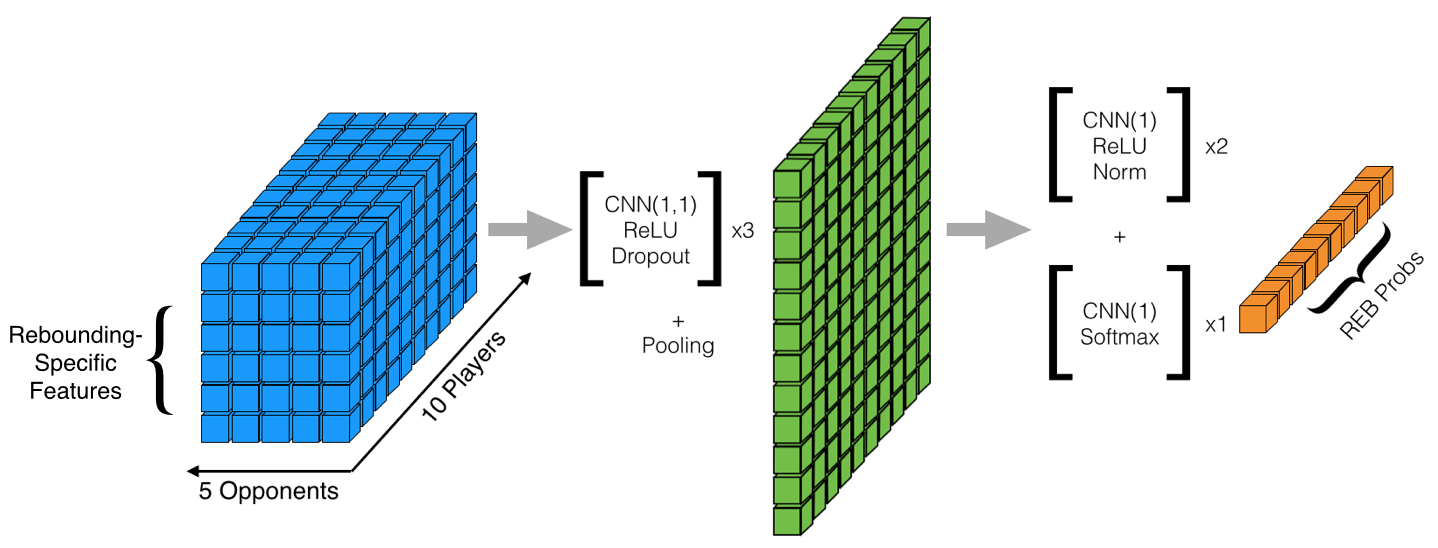
\includegraphics[width=1\columnwidth]{Modeling_Process.png}
\caption{\bf{Simplified ReboundNet Structure}}
\label{fig:Modeling_Process}
\end{figure}

\bigbreak
\noindent
In \textcolor{blue}{Figure} \ref{fig:Modeling_Process} above, only the rebounding-specific features 1--3 vary along the opponents dimension of the input tensor. The first block of convolutions learns to work with each pair of opposing players. Specifically, this block of convolutions learns interactions such as boxouts and close--outs on shooters. The second block of convolutions focuses on each player individually, and finishes with a softmax activation to output the probability of each individual player recording a rebound on the play.

\bigbreak
\noindent
A key attribute of this network structure is that it is not dependent on the order in which the players are inputted. The convolutions and pooling used ensure that the model predictions are the same regardless of the order in which the data is inputted.

\subsection{Model Training}
\noindent
The full set of 33,089 rebounding plays available from the data were split into training, validation, and holdout groups. The training data was augmented to include a spatially flipped version of each play\footnote{By "flipped version", we mean that we alter the positions of each player to become what the positions would be at the opposite end of the court.}, assuming that each of the rebounding plays would have had the same outcome in a mirrored world. This resulted in a training data set with 46,000 plays, and validation and holdout groups with 5,000 plays.

\bigbreak
\noindent
The training data set was fed to the ReboundNet structure shown in \textcolor{blue}{Figure} \ref{fig:Modeling_Process}. The loss function considered the rebounding probabilities both at a player and team level, by averaging the binary cross--entropy of team level predictions with the absolute error of player level predictions\footnote{The absolute error was used for player level predictions in place of categorical cross--entropy, because the latter was shown to systematically over predict small rebound probability values.}. ReboundNet's predictions were tested against the 5,000 holdout sample plays (which ReboundNet never saw during training!). On this holdout data, ReboundNet assigned the highest rebounding probability to the player who eventually recorded the rebound 49\% of the time. For perspective, if you guessed the player closest to the estimated landing spot of the ball to be the eventual rebounder, you would be correct 37\% of the time. As a result, ReboundNet offers about a 33\% improvement in accuracy over educated guessing. Additionally, one of the top 3 players scored by ReboundNet in a play obtained the rebound 79\% of the time.

\subsection{Model Interpretation}

The best way to understand how ReboundNet works is to examine specific examples.

\begin{figure}[htb]
\centering
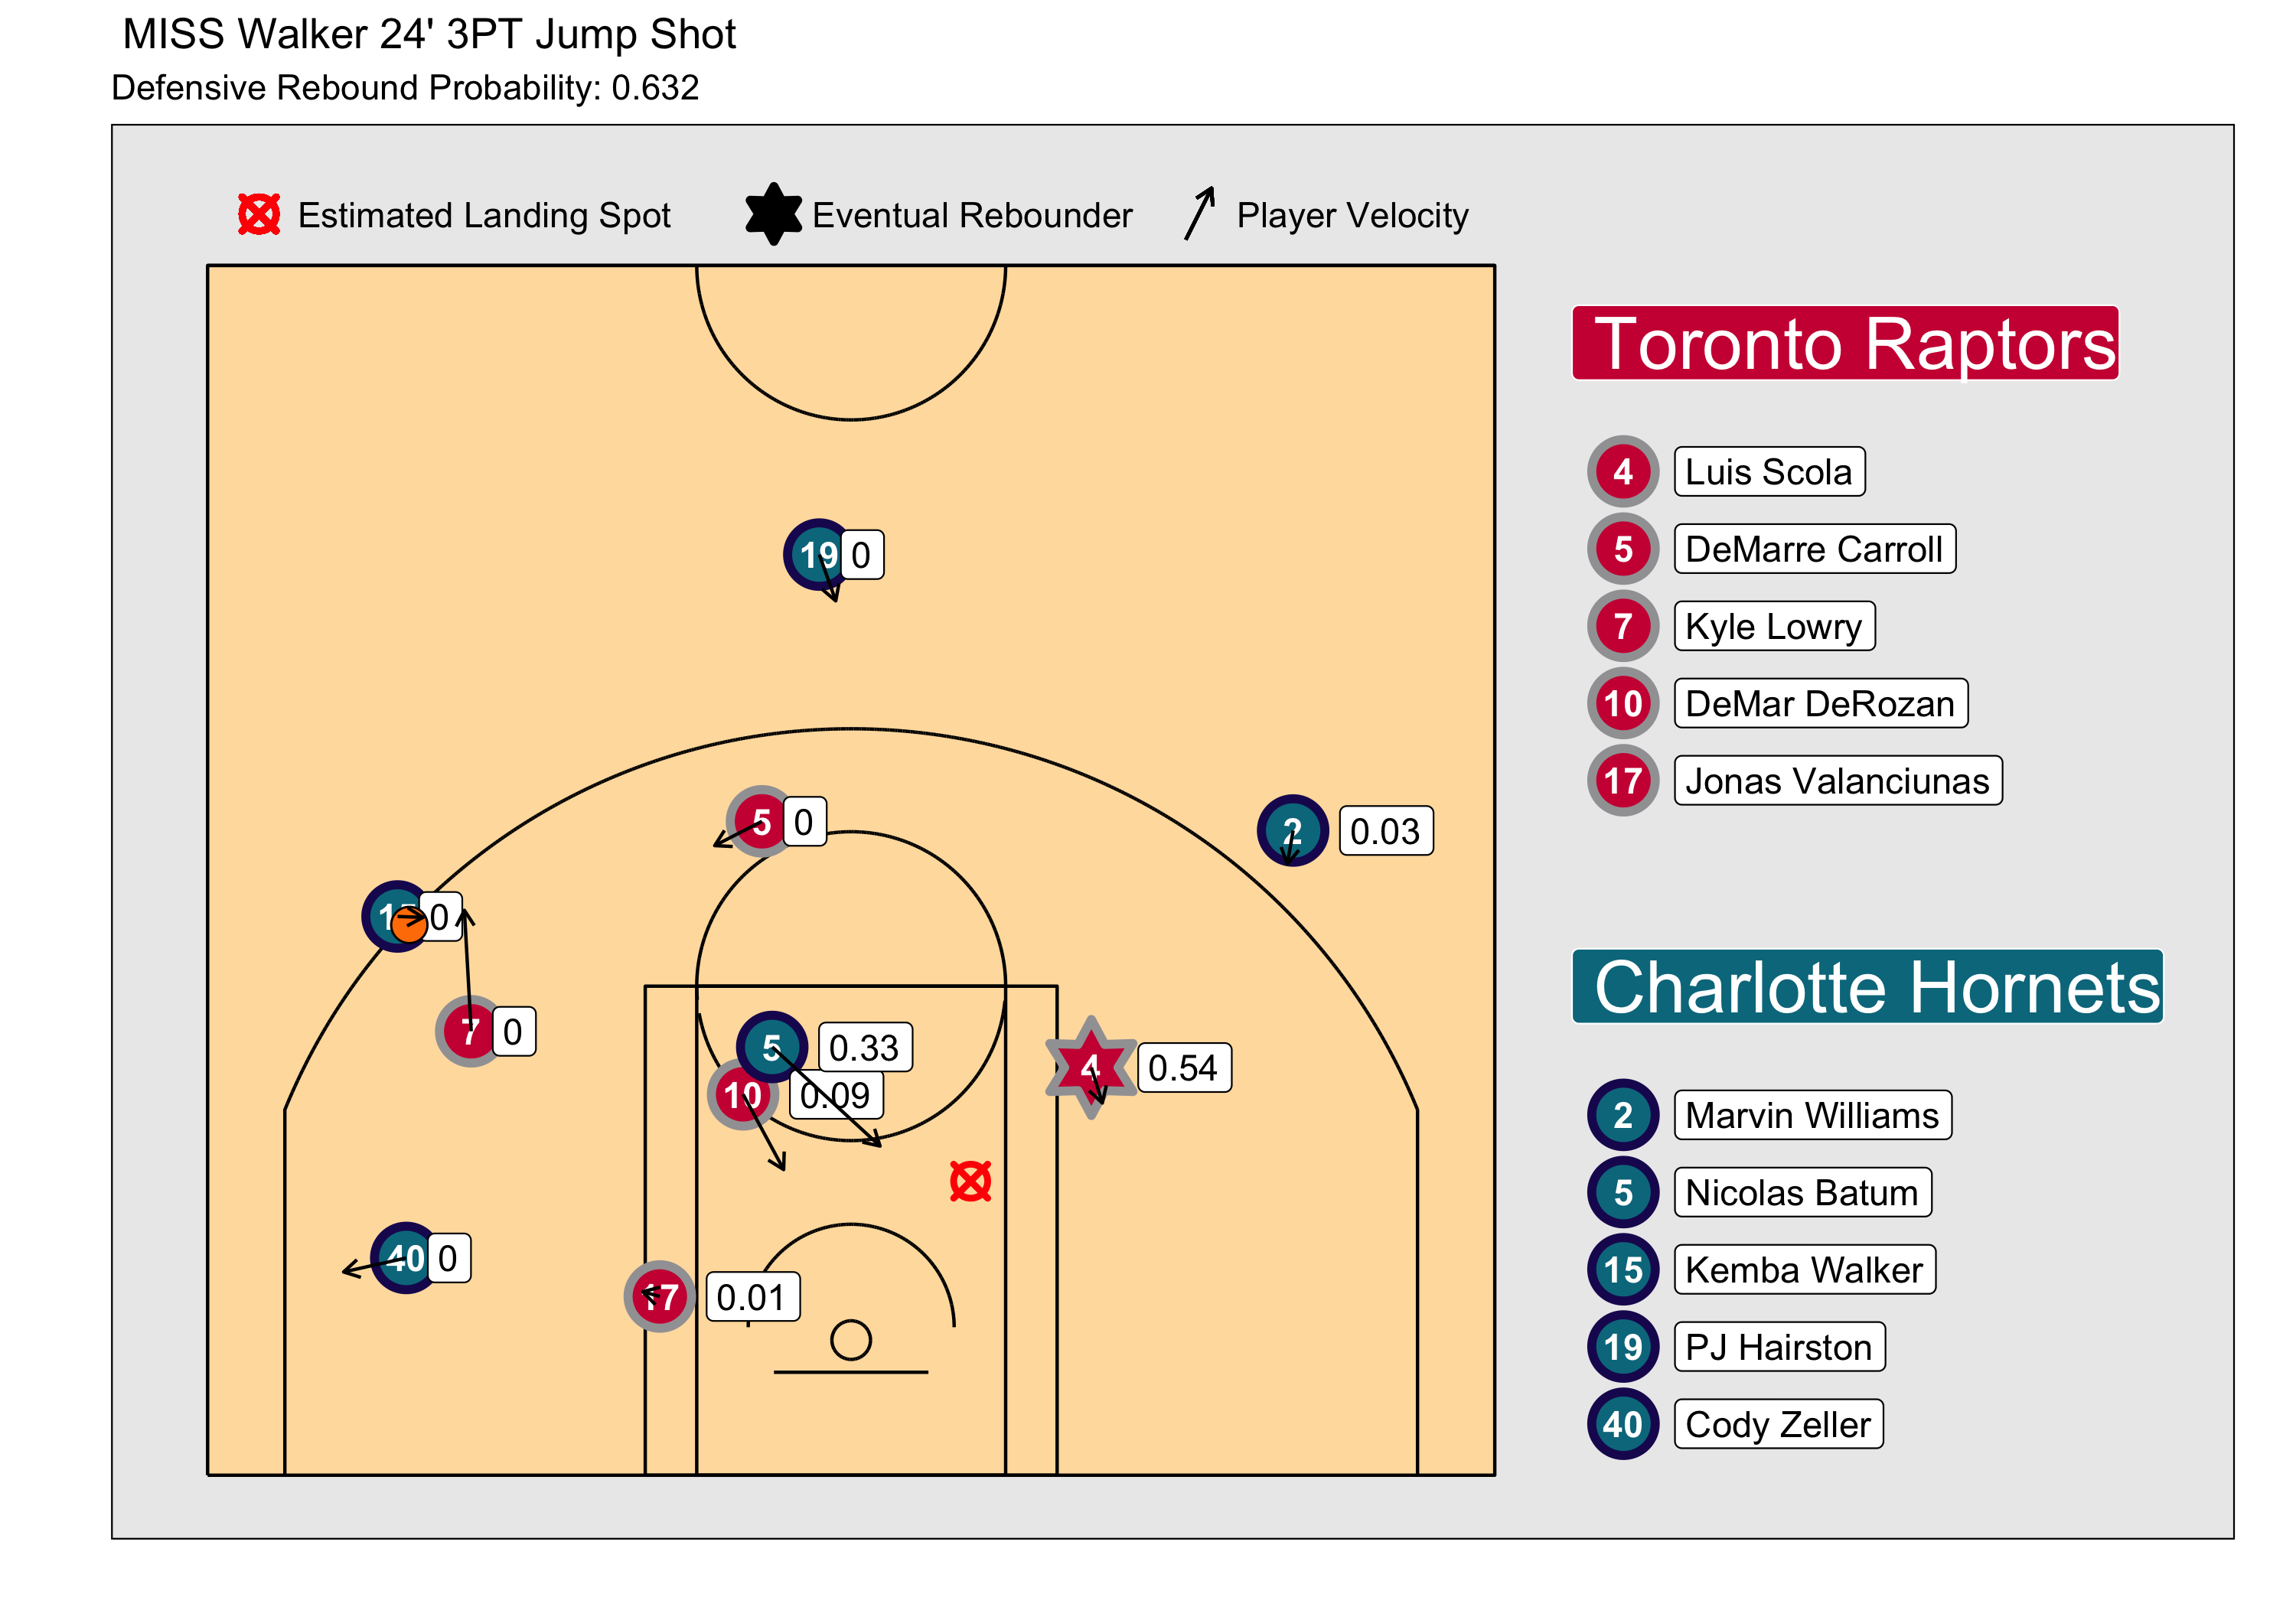
\includegraphics[width=1\columnwidth]{ReboundEx.png}
\caption{\bf{Example Rebounding Play With ReboundNet Probabilities}}
\label{fig:ReboundEx}
\end{figure}

\noindent
\textcolor{blue}{Figure} \ref{fig:ReboundEx}, above, shows the rebound probabilities that ReboundNet assigns to each player for the play shown in \textcolor{blue}{Figure} \ref{fig:ReboundExNoProbs}. From this example, we can begin to see the importance of the expected landing spot on the predictions made by ReboundNet. The three closest players to the expected landing spot (Luis Scola, Nicolas Batum, and DeMar DeRozan), have a combined rebound probability of 96\%. In fact, while there are other factors ReboundNet considers (as will be discussed shortly), the singular most important factor influencing a player's rebound probability is their distance from the expected landing spot. 

\bigbreak
\noindent
\textcolor{blue}{Figure} \ref{fig:LandingEx}, below, provides a more extreme example showing the importance of proximity to the expected landing spot.

\begin{figure}[htb]
\centering
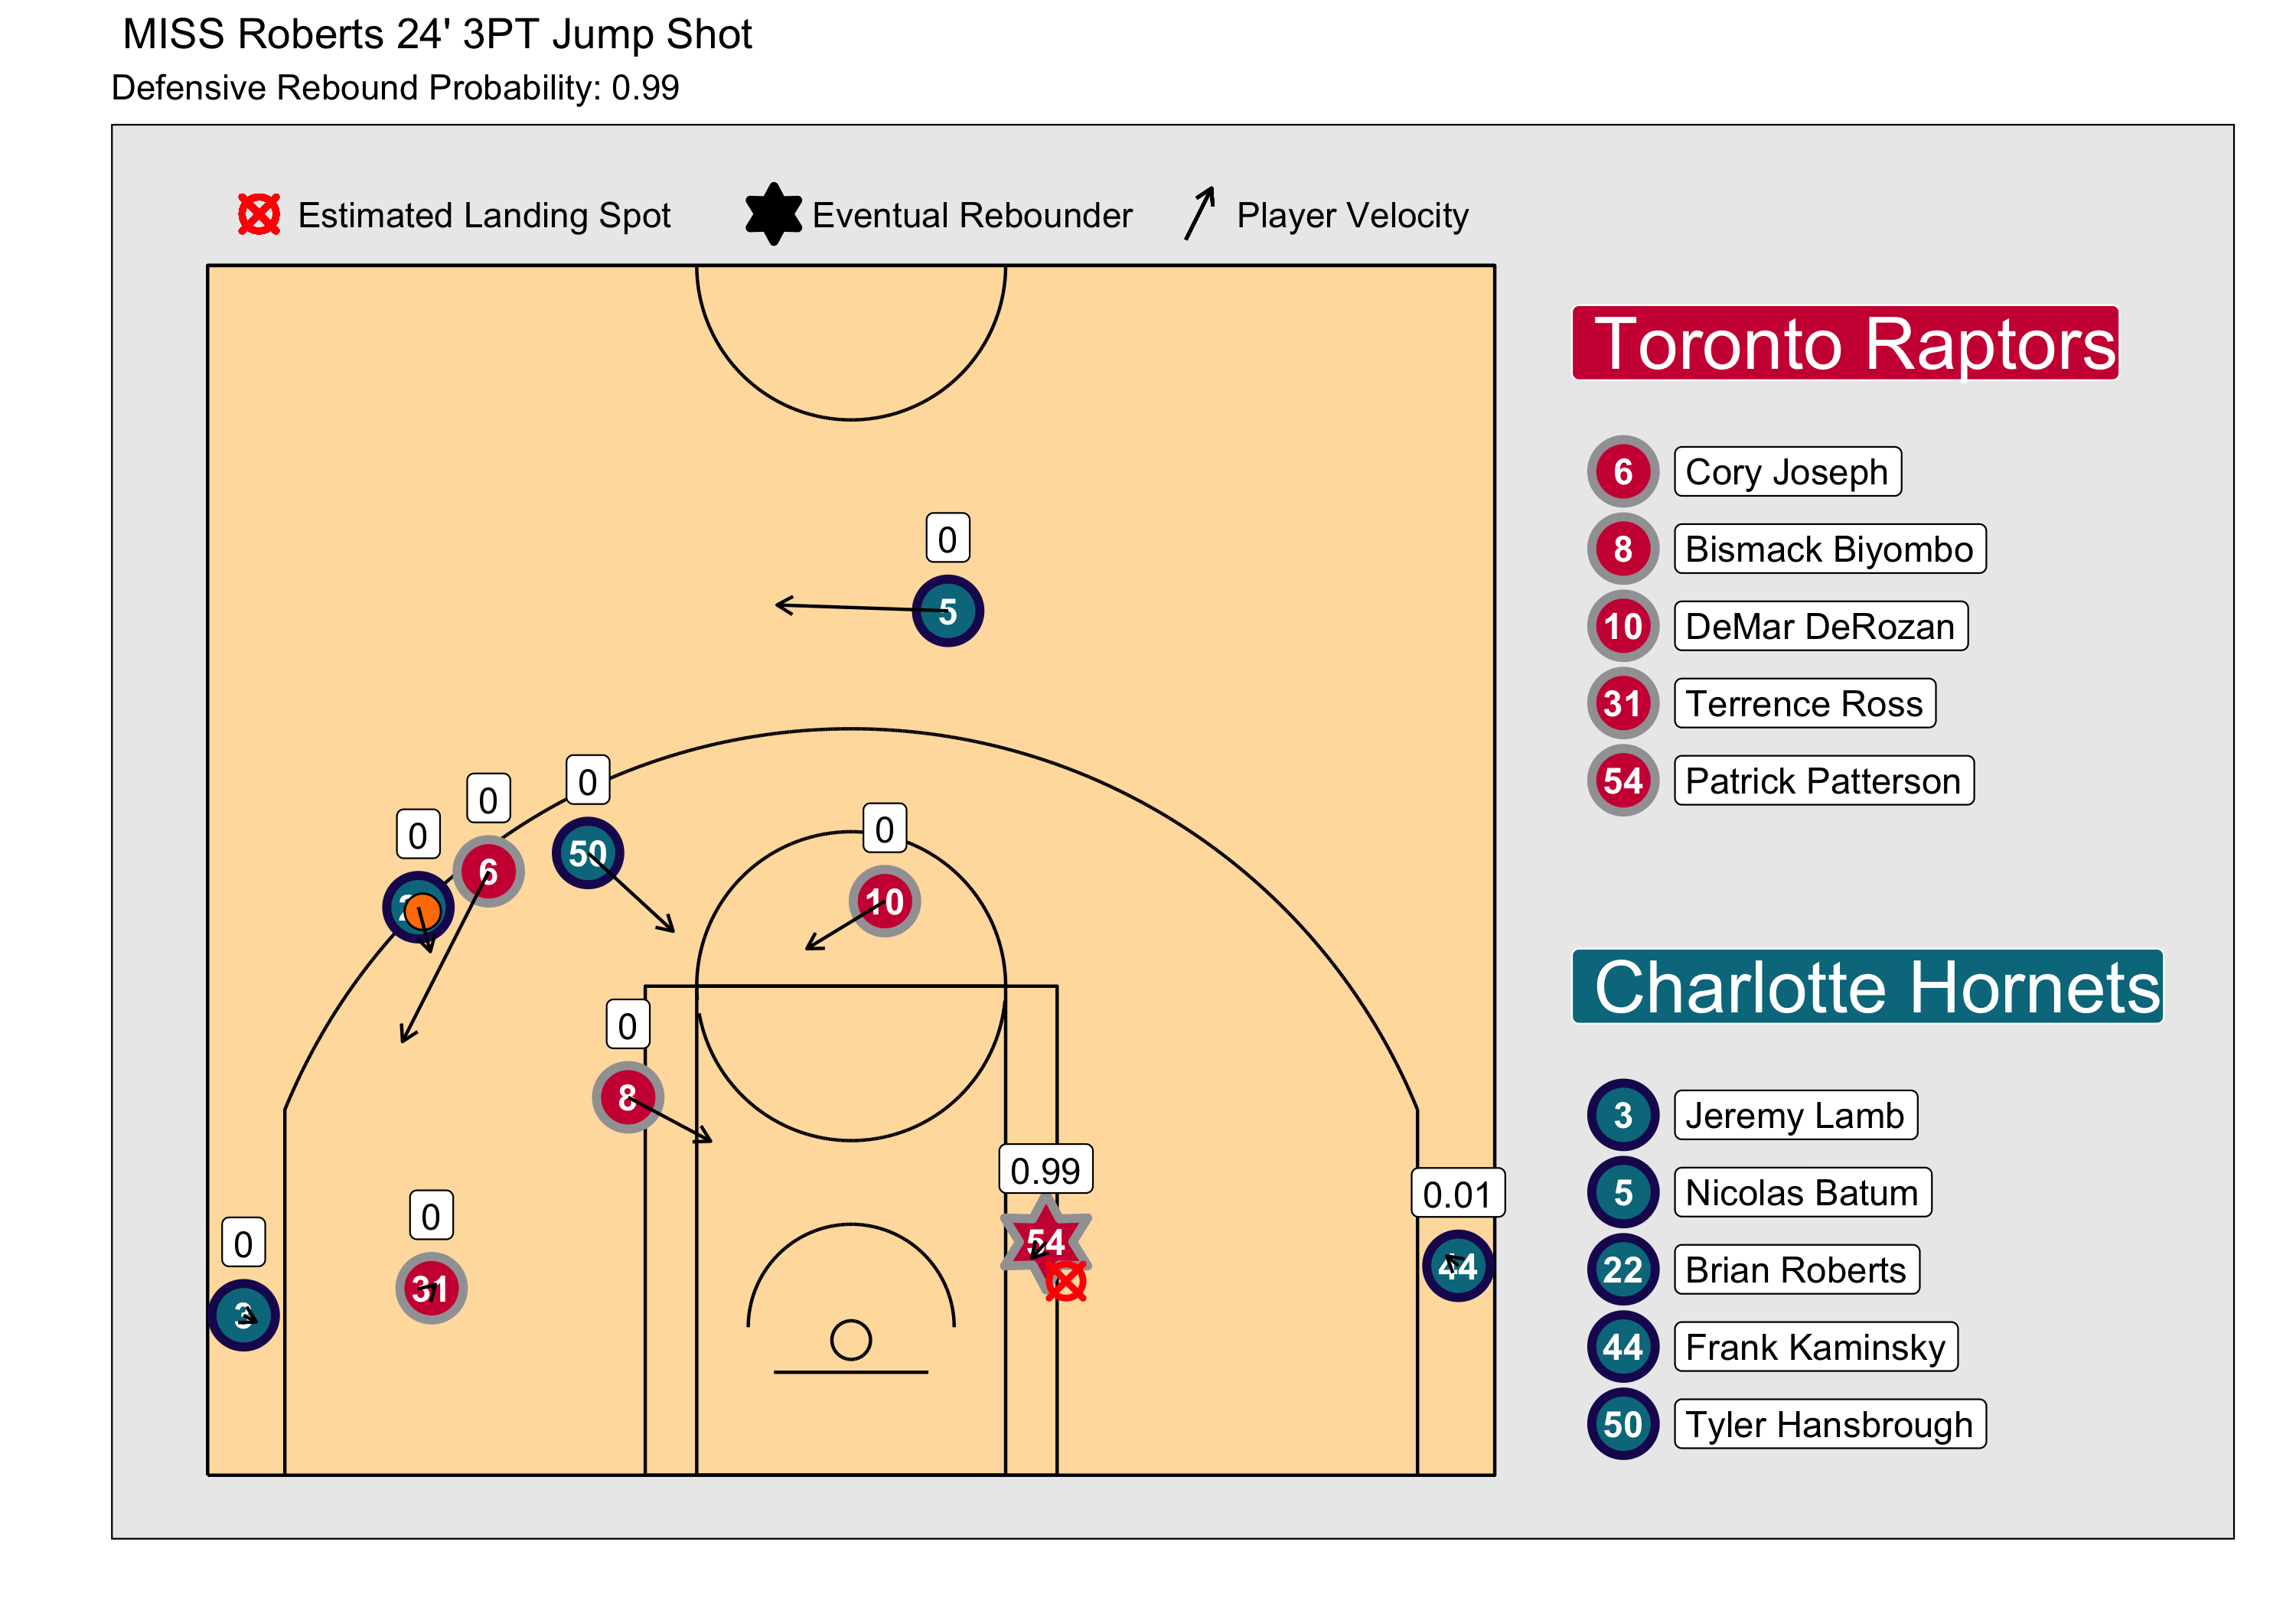
\includegraphics[width=1\columnwidth]{LandingEx}
\caption{\bf{Importance of Proximity to Expected Landing Spot}}
\label{fig:LandingEx}
\end{figure}

\bigbreak
\noindent
As can be seen above, ReboundNet is already chalking up the rebound to Patrick Patterson at the time of the shot, given knowledge of the ultimate landing spot of the basketball. Why is it doing this? In this instance, Patrick Patterson is the only player within a 15 foot radius of the ultimate landing spot. As a result, he would have to either horribly misjudge the ball, trip, or not catch the rebound cleanly to avoid rebounding the basketball. In this case, ReboundNet is aggressive, and assigns almost a 100\% rebound probability to Patrick Patterson. 

\bigbreak
\noindent
So far, we have seen that ReboundNet is great at figuring out which players are closest to the expected landing spot of the ball, and assigning these players the highest rebound probabilities. But ReboundNet is actually processing much more than just this. Recall the different rebound--specific features that ReboundNet considers, and that ReboundNet offers approximately a 33\% improvement in prediction accuracy above guessing the rebounder to be the player closest to the expected landing spot of the ball. ReboundNet is able to offer such an improvement in accuracy by considering all of the rebound--specific features identified above, and determining informative patterns from these features that impact rebound probabilities.

\bigbreak
\noindent
One such informative pattern is simply the box--out interaction. ReboundNet is able to identify when one player is boxing out an opponent. Additionally, it is able to infer the relative strength of the box--out, and lower the rebounding probability of the player being boxed out accordingly. Consider \textcolor{blue}{Figure} \ref{fig:BoxOutEx} below.

\begin{figure}[htb]
\centering
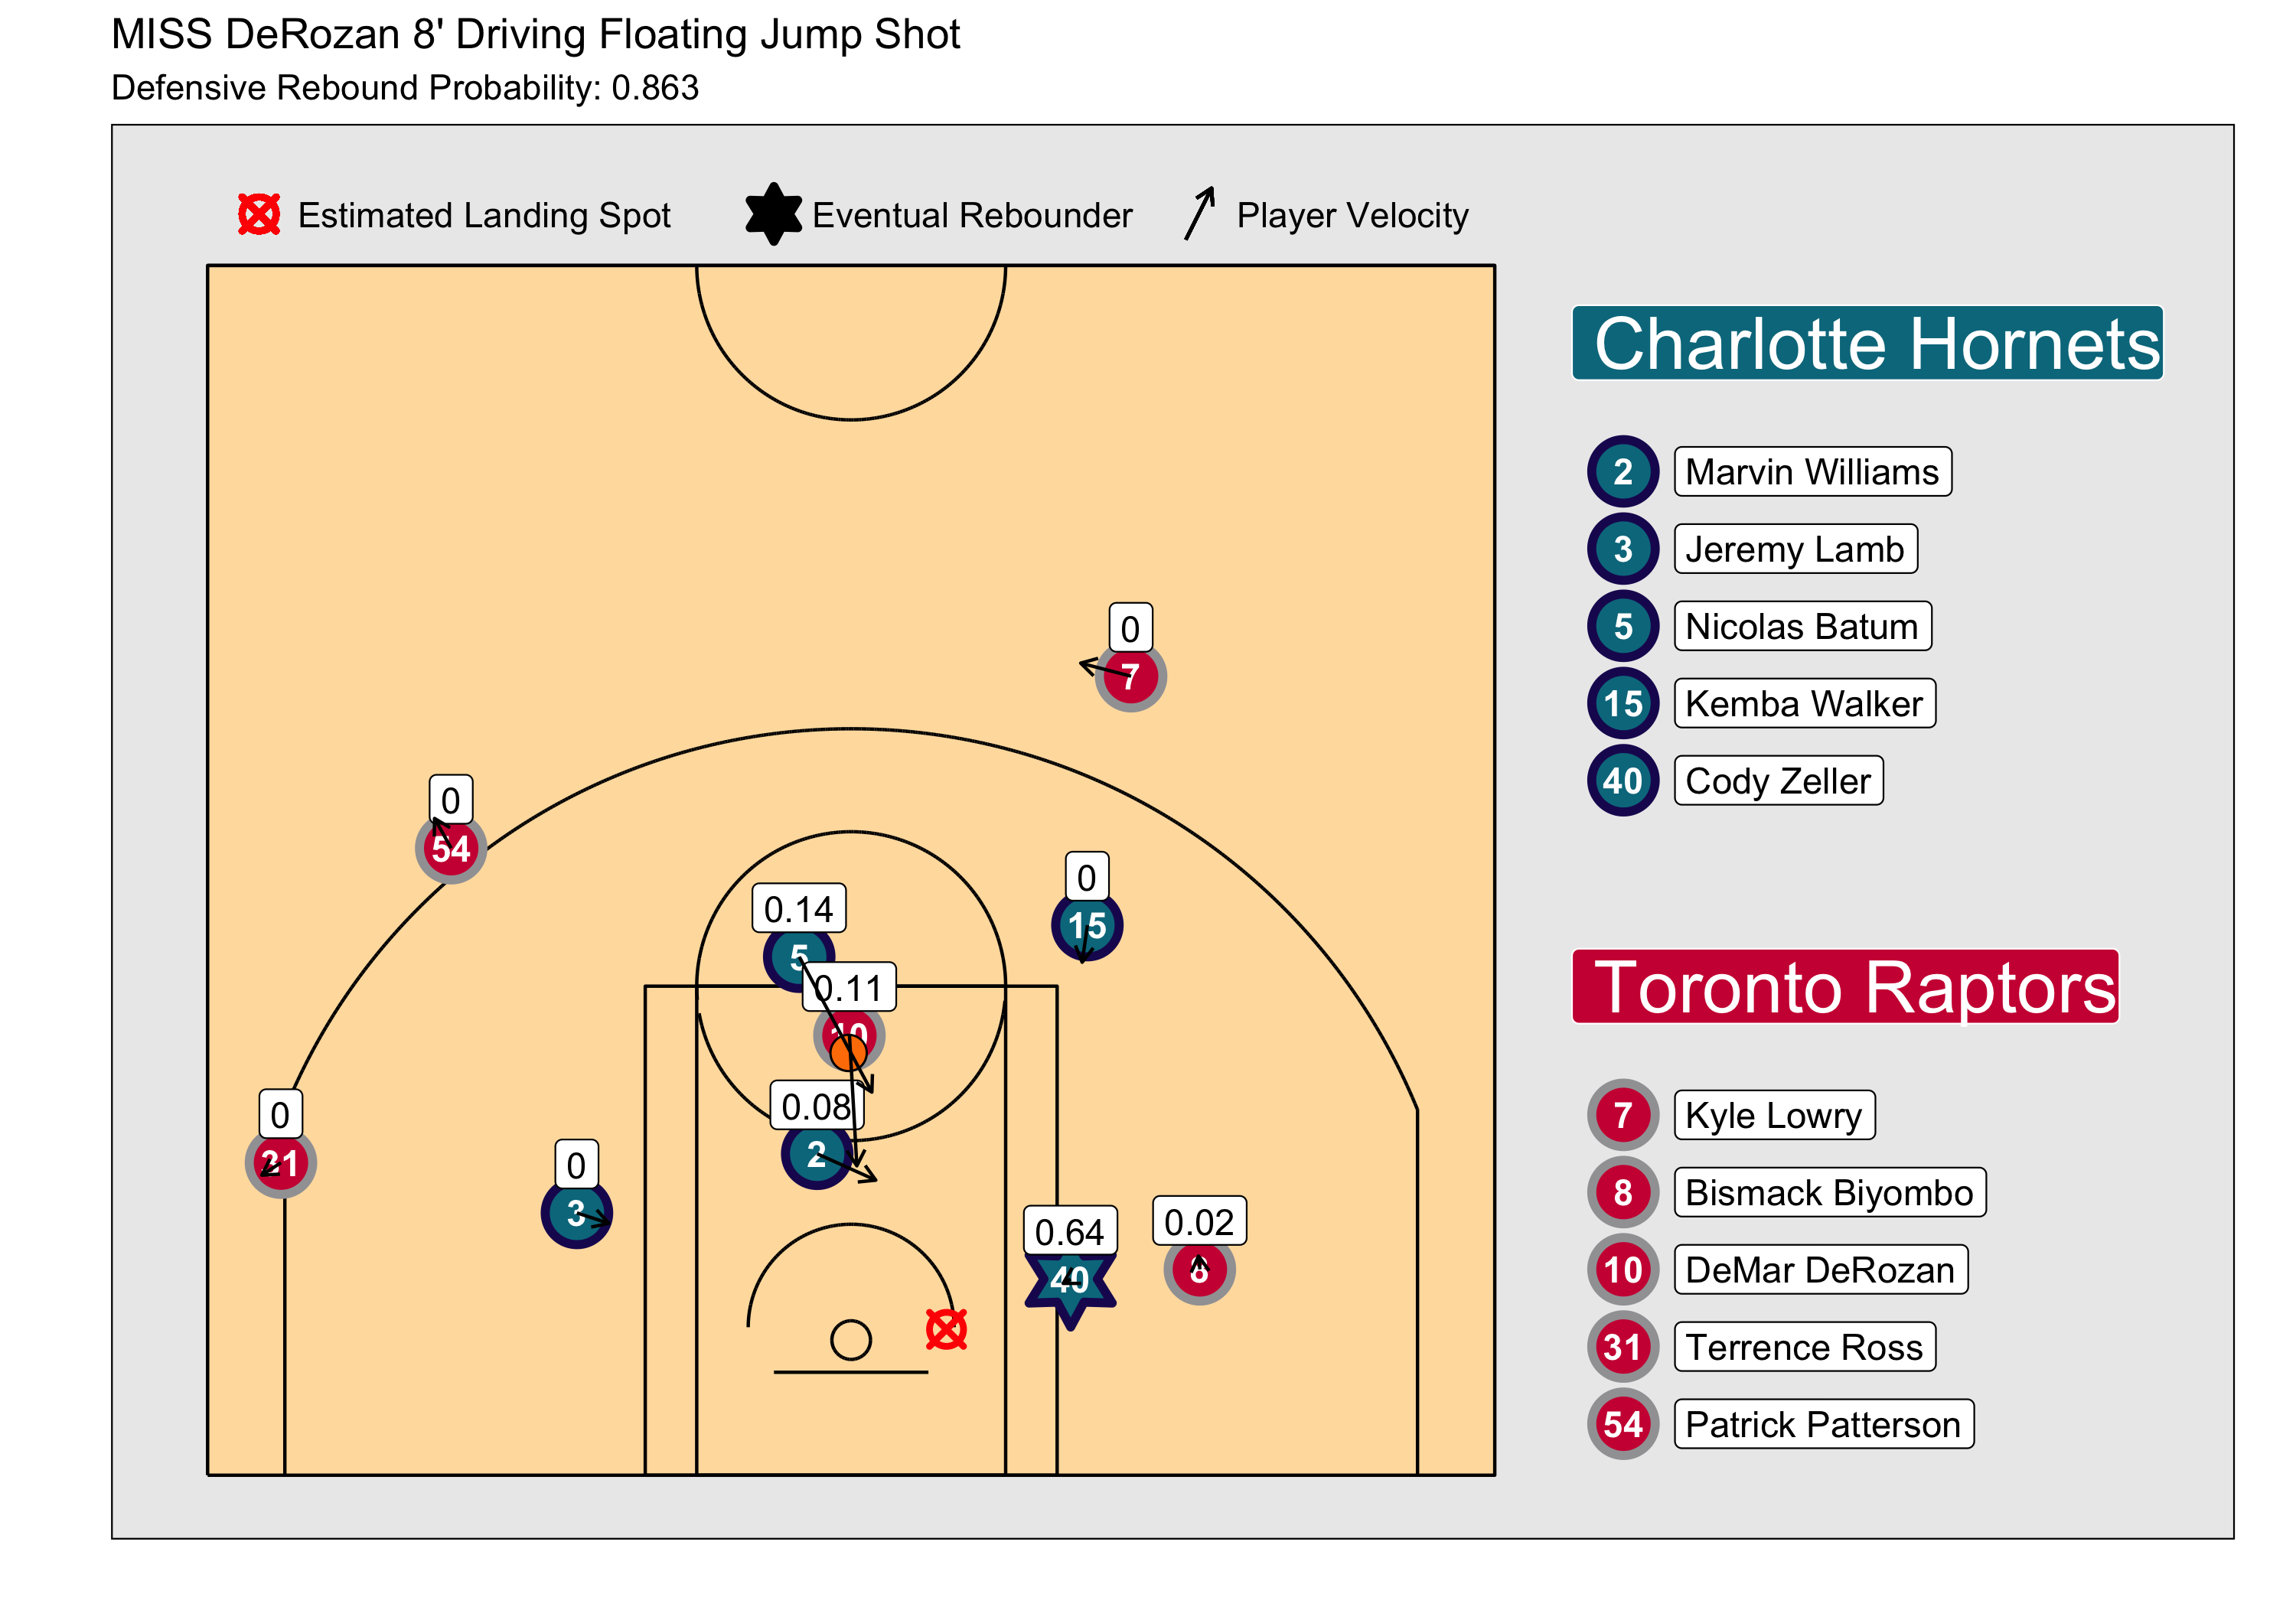
\includegraphics[width=1\columnwidth]{BoxOutEx.png}
\caption{\bf{Identification of Box--Out Interaction}}
\label{fig:BoxOutEx}
\end{figure}

\noindent
On this play, since ReboundNet knows that Cody Zeller is in between Bismack Biyombo and the hoop (and that these players are opponents), it identifies a boxout situation. As a result, Bismack Biyombo's rebound probability is much lower than it would usually be given his distance from the expected landing spot of the ball. As a point of comparsion, Marvin Williams is four times more likely to record a rebound on this play than Bismack Biyombo according to ReboundNet, despite both players being about the same distance away from the expected landing spot. The key difference is that Marvin Williams has no opponents in between his path to the ball, but Bismack Biyumbo is being boxed out by an opponent.

\bigbreak
\noindent
But ReboundNet can identify more than just box--out situations. Another common interaction that ReboundNet can identify is a close--out by a defender. Such a play commonly occurs when a defender rushes towards a shooter to contest a shot. In doing so, the defender is taking themselves out of rebounding position, as they are moving quickly away from the hoop. \textcolor{blue}{Figure} \ref{fig:SpeedEx}, below, gives an example of how ReboundNet accounts for close--outs. 

\clearpage

\begin{figure}[htb]
\centering
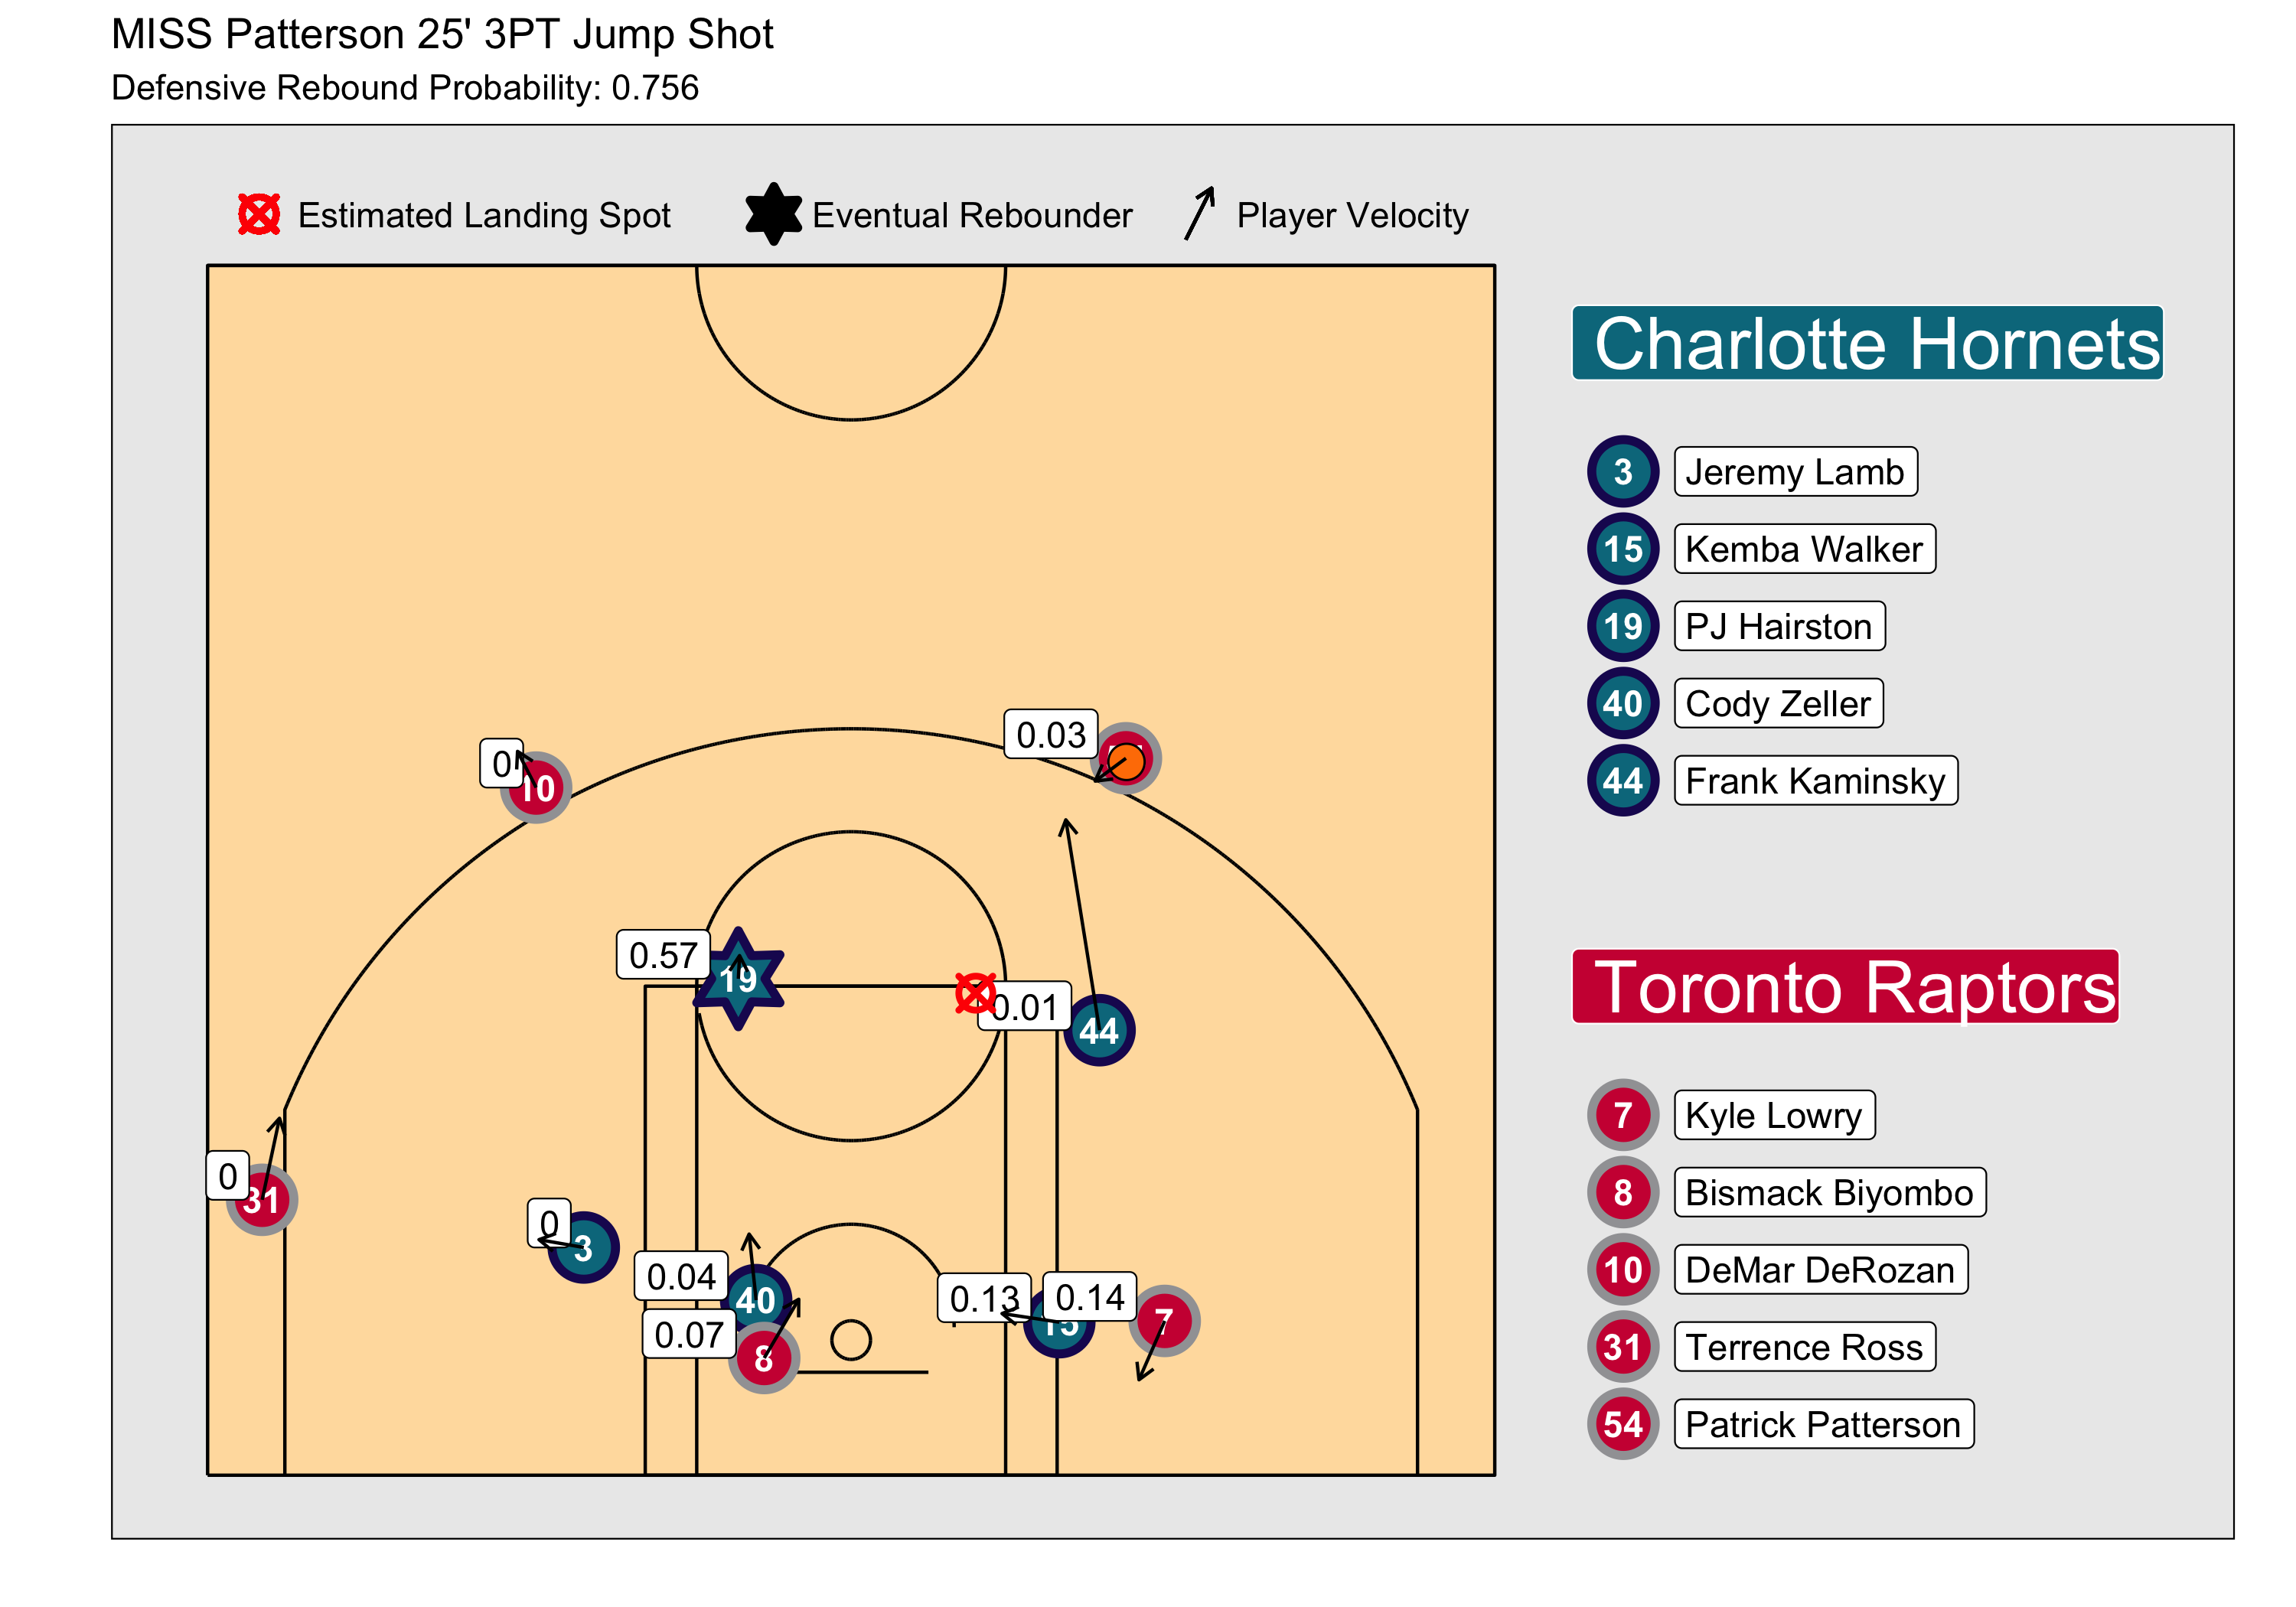
\includegraphics[width=1\columnwidth]{SpeedEx.png}
\caption{\bf{Identification of a Close--Out}}
\label{fig:SpeedEx}
\end{figure}

\noindent
On this play, Frank Kaminsky is closing out on the shooter, Patrick Patterson. As shown in the diagram, Kaminsky is moving very quickly towards Patrick Patterson to contest his shot. ReboundNet takes this into consideration when assigning Frank Kaminsky his rebound probability. Somewhat amazingly, despite being the closest player to the expected landing spot of the shot, Kaminsky is assigned a slim 1\% rebound probability. This indicates ReboundNet has identified through the many plays it analyzed that defenders closing out on a shooter are very unlikely to record a rebound. As a result, ReboundNet correctly assigns the next closest player, PJ Hairston, the highest rebound probability.

\bigbreak
\noindent
ReboundNet is able to identify more patterns than just box--outs and close--outs, but understanding how it is able to quantify those two patterns helps to build intuition on how ReboundNet assigns rebound probabilities to each player. The above plots are certainly interesting to analyze by themselves, but we can go beyond looking at single plays to make the analysis more interesting. Specifically, by aggregating plays at the team or player level, the results of ReboundNet can be used to produce rebound ratings at the team and player level. This is the focus of the next section.

\clearpage

\section{ReboundNet Evaluation Metrics}

\subsection{Team Evaluation}
\noindent
Throughout the course of the season, it is commonly wondered how teams compare in terms of rebounding ability. This is commonly answered by looking at metrics like rebounds per game (or per opportunity) at a team level. But as we have seen, not all rebounding opportunities are created equally. Some teams may benefit from favorable shot landing spots, while others may inherit less opportune situations. It is desirable to have a metric that accounts for such circumstance, to fairly rate the rebounding ability of each team independent of their inherited situations\footnote{Part of a team's inherited circumstance is their own doing. If a team really prioritizes rebounding, its players may crash the boards more frequently on offensive possessions, or more stringently stay between their man and the basket on defensive plays. ReboundNet only considers activity after the time of the shot, and in doing so ignores these effects.}.

\bigbreak
\noindent
The predictions made by ReboundNet enable such a metric. Since ReboundNet tabulates rebounding probabilities for all 10 players on the court, these probabilities can be summed at the team level to provide team rebounding probabilities. Such probabilities were provided for the defensive team in the title of \textcolor{blue}{Figures} \ref{fig:ReboundEx}\textcolor{blue}{--}\ref{fig:SpeedEx}. 

\bigbreak
\noindent
These probabilities enable us to analyze how a team rebounded against how it was expected to rebound. Take the play in 
 \textcolor{blue}{Figure} \ref{fig:SpeedEx} as an example. The Charlotte Hornets were estimated by ReboundNet to have a 75.6\% chance of recording a rebound on this play. Statistically speaking, this means the Hornets expected number of rebounds to come out of this play was 0.756 rebounds\footnote{Of course, a team either does or does not record a rebound, so there is no notion of a partial rebound. This can be interpreted to mean that if the play was simulated a million times, Charlotte would get the rebound about 75.6\% of the time.}. Additionally, we know that Charlotte did record a rebound on this play. Given ReboundNet's prediction, we can claim that Charlotte added 0.246 rebounds above expectation. Conversely, Toronto is debited 0.246 rebounds on the play, since they were expected to get 0.246 rebounds and got none.
 
 \bigbreak
\noindent
This may seem like an odd way to analyze rebounds at first. Charlotte recorded a rebound on the play, so why are they only getting credit for 0.246 rebounds? It makes more sense when recalling the play in \textcolor{blue}{Figure} \ref{fig:LandingEx}. On this play, since the ball bounces right at an isolated Patrick Patterson, it was unimpressive that Toronto recorded a rebound on this play. That rebound should barely (if at all) change our opinion Toronto's rebounding ability. ReboundNet accurately captures this, as it assigned the Raptors a 99.0\% chance of recording a rebound. Following our logic from above, this means we can claim that Toronto added 0.01 rebounds above expectation on this play. This is an insignificant boost, and aligns with common sense logic that Toronto should not be credited much for getting such an easy rebound.
\bigbreak
\noindent
Mathematically, we can define a team's net rebounds added per play as the following: Let $P^{Reb}_{ij}$ be defined as the probability of team $i$ getting a rebound on their $j$th opportunity. Let $\mathds{1}^{Reb}_{ij}$ be 1 if team $i$ records a rebound on play $j$ and 0 otherwise. Then if team $i$ had $n_{i}$ total rebounding opportunities in a season,

$$ \text{NetREB}_{i} = \frac{\sum_{j=1}^{n_{i}}(\mathds{1}^{Reb}_{ij} - P^{Reb}_{ij})}{n_{i}} $$

\noindent
where  $\text{NetREB}_{i}$ is the net rebounds above expectation that team $i$ records per play, adjusting for the hand team $i$ was dealt in terms of shot landing spots and player locations over its rebounding opportunities.
\bigbreak
\noindent
From the player tracking data provided, we were able to compute this metric for all 30 teams based on their performance in the first half of the 2015--2016 NBA season. A summary of the 5 best and worst teams is provided below in \textcolor{blue}{Table} \ref{table:TeamScores}. The values are scaled to 100 opportunities to make the results more interpretable (there are around 100 rebounding opportunities in total per game), where $\text{NetREB}^{100}_{i}$ is team $i$'s net rebounds added over 100 opportunities.

\renewcommand{\arraystretch}{1.0}
\begin{table}[htb]
  \centering
  \caption{Team Net Rebounds Added Per 100 Opportunties from the 2015--2016 NBA Season}\label{table:TeamScores}
  \begin{tabular}{cccccc}
  \toprule
 &\multicolumn{1}{c}{{\it Best}}
&
\multicolumn{4}{c}{{\it \quad \quad \quad Worst}} \\  \cmidrule(r){2-2}\cmidrule(l){5-5}
Rank & Team & $\text{NetREB}^{100}$ & Rank & Team & $\text{NetREB}^{100}$ \\
	\midrule
	1 & Detroit Pistons & {\bf \textcolor{ForestGreen}{+2.66}} & 30 & Milwaukee Bucks & {\bf \textcolor{BrickRed}{--2.26}}  \\
	2 & Cleveland Cavaliers & {\bf \textcolor{ForestGreen}{+2.03}} &  29 & Philadelphia 76ers & {\bf \textcolor{BrickRed}{--1.86}}  \\
	3 & Oklahoma City Thunder  & {\bf \textcolor{ForestGreen}{+1.97}} &  28 & Los Angeles Lakers & {\bf \textcolor{BrickRed}{--1.51}} \\
	4 & Toronto Raptors  & {\bf \textcolor{ForestGreen}{+1.56}} & 27 & Memphis Grizzlies & {\bf \textcolor{BrickRed}{--1.41}} \\
	5 & Denver Nuggets & {\bf \textcolor{ForestGreen}{+1.49}} & 26 & New York Knicks & {\bf \textcolor{BrickRed}{--1.40}} \\
\bottomrule
  \end{tabular}
\end{table}

\bigbreak
\noindent
We can also analyze teams rebounding ability on the offensive and defensive ends. Offensive and defensive rebounding situations are distinct in nature. The offensive rebounder is playing on the team of the shooter, and may potentially know exactly when a shot is going to go up (by knowing the play call or player tendencies). However, the defensive team has an advantage, since the offensive shooter essentially makes the rebounding play a 5 on 4 in favor of the defense. Additionally, defensive players tend to be positioned between the basket and the player they are guarding, leaving them in more favorable rebounding position. Strategy also impacts offensive rebounding. Some teams are aggressive on the offensive boards, prioritizing the chance at an extra possession at the expense of potentially giving up an easy transition bucket, while others are more conservative.

\bigbreak
\noindent
These factors lead to 81\% of the rebounding opportunities in the sample studied going in favor of the defense. \textcolor{blue}{Figure} \ref{fig:TeamsPlot}, below, breaks out each team's rebounding performance by offensive and defensive team rebounds added per 100 possessions.


\begin{figure}[htb]
\centering
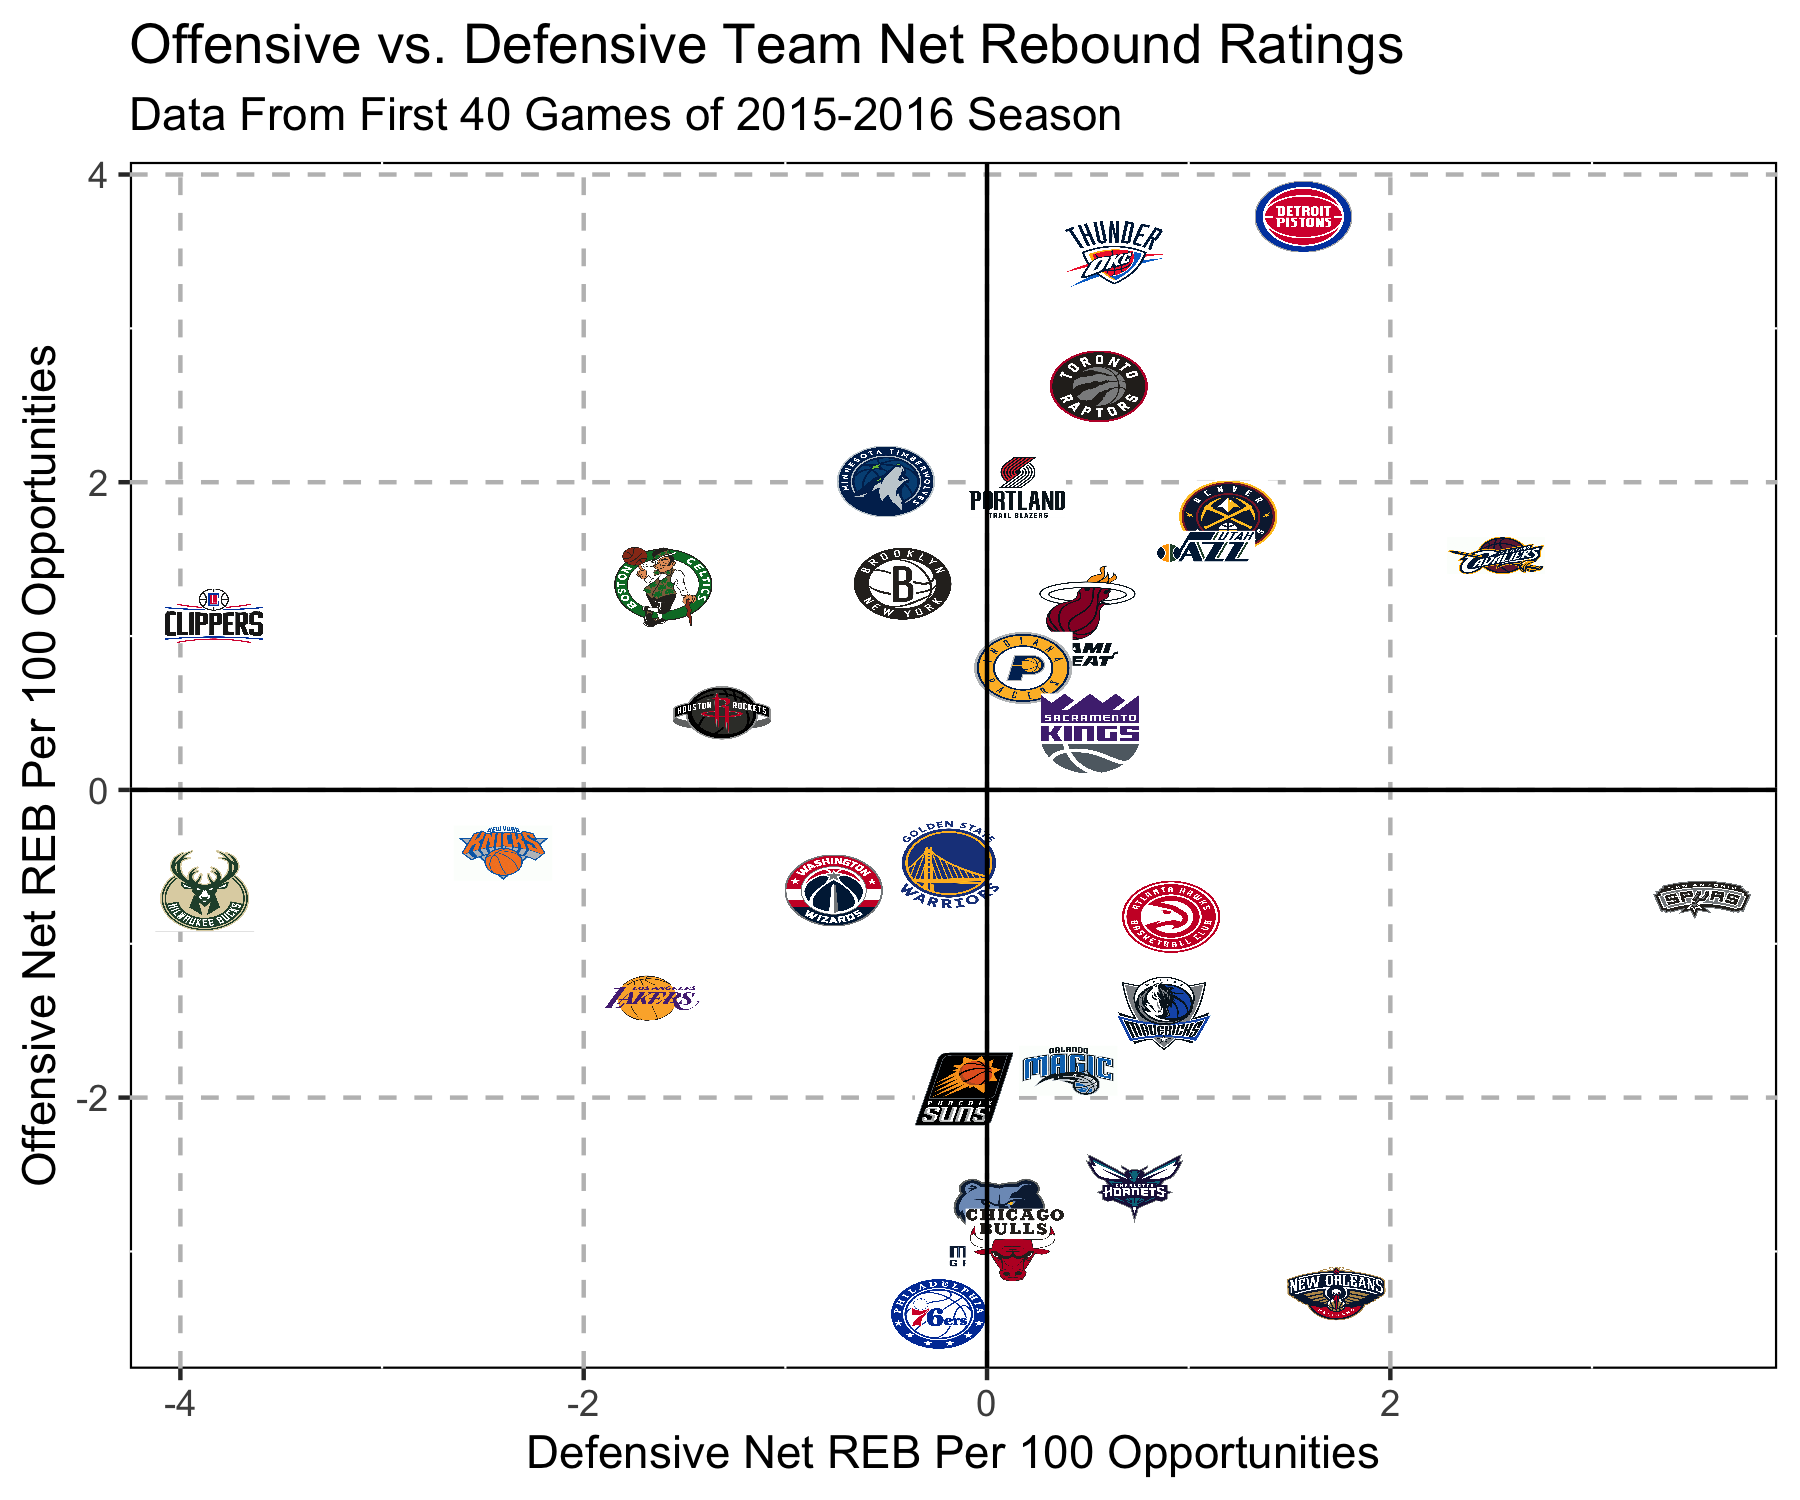
\includegraphics[width=.8\columnwidth]{TeamsPlot.png}
\caption{\bf{Comparison of Offensive and Defensive Net Rebounds By Team}}
\label{fig:TeamsPlot}
\end{figure}

\noindent
Some teams were poor offensive and defensive rebounding teams, such as the New York Knicks and the Los Angeles Lakers. Others, such as the Detroit Pistons and the Cleveland Cavaliers, were great offensive and defensive rebounding teams. The San Antonio Spurs are interesting, as they were the best defensive rebounding team but a below average offensive rebounding team. This may have been a result of strategy -- as noted earlier, it is possible the Spurs were prioritizing transition defense and keeping the pace of the game slow over the potential extra possession earned by crashing the offensive boards. The Houston Rockets may have been the converse to the Spurs.Their gunslinger 3--point mentality, combined with a propensity to crash the offensive boards, resulted in Houston being an above average offensive rebounding team, despite being below average at the defensive end.

\subsection{Player Evaluation}
\bigbreak
\noindent
The rebounding ability of a player impacts his value. Fans often argue over who the best rebounders in the game are, and front offices take into account the rebounding ability of players when considering potential transactions. As a result, it would be beneficial to create a player rebounding metric, just as we did for teams. Using the results of ReboundNet, we can do just that.

\bigbreak
\noindent
At first, it seems as though the metric measuring player rebounding ability should be analogous to our metric measuring team rebounding ability. Just like for team rebounding where we measure how a team rebounded against its rebounding probabilities, we similarly can measure how a player rebounded against his own rebounding probabilities. But there is a critical flaw in this formulation: the value of a rebound should never be viewed at the player level, but rather always at the team level. 

\bigbreak
\noindent
Why is this the case? Once again consider the extreme example shown in \textcolor{blue}{Figure} \ref{fig:LandingEx}. Imagine that Bismack Biyombo soared in at lighting speed, and grabbed the rebound in front of the outstretched arms of Patrick Patterson. Applying our logic from the team rebounding metrics, we would argue that since Bismack Biyombo was given approximately a 0\% chance of recording the rebound, he would have gained a full net rebound on the play. The issue is that this net rebound came at the expense of his teammate, Patrick Patterson, who we would say lost a net .99 rebounds on the play. Clearly, all Bismack Biyombo did on this play was cannibalize a rebound his teammate would have recorded anyways\footnote{While this example may seem contrived, it occurs more often that one would think at first glance. Often times, players will "steal" rebounds from their teammates in an effort to increase their rebounding total. This occurs most commonly to secure a triple--double, but also when a high volume rebounder is close to a guard who lets them record a rebound.}, so he should not be awarded much value for his efforts.

\bigbreak
\noindent
While the example discussed is an extreme, this same effect occurs on every rebounding play. We would be over--stating a player's impact on the game by looking at how he shifted his own rebounding probabilities, since his teammates also have some chance at rebounding the basketball! To correct for this, we argue that the rebounder for a given play should be credited with the probability the opposing team had of recording a rebound on the play. In this way, we ignore any cannibalized probabilities, and only credit the rebounder with the probability that he took from his opponents. Referencing \textcolor{blue}{Figure} \ref{fig:LandingEx}, this means that if Bismack Biyombo would have recorded the rebound, he would only be awarded 0.01 net team rebounds added on the play, since this was the probability given to Charlotte (his 5 opponents) of recording a rebound on the play.
 
\bigbreak
\noindent
Now we know how to account for the rebounder, but what about the other 9 players? The goal for each player in any rebounding play is for his team to secure the rebound. As a result, the other 4 players on the rebounding team succeeded in this goal, so they should not be docked any net rebounds. We argue these four players should not be debited or credited any value at all. On the other hand, the 5 players on the non--rebounding team should be debited the rebounding probabilities assigned to them by ReboundNet. This is because each player on the non--rebounding team cost their team this many rebounds. This leads to the nice result that for any given rebounding play, the sum of the net team rebounds credited and debited from all 10 players is 0.

\clearpage
\noindent
We can formulate these scores mathematically as follows. Let $\hat{P}^{Reb}_{i}$ be defined as the probability of player $i$ getting a rebound for a fixed play. Let $P^{OppReb}_{i}$ be defined as the probability of the opposing team of player $i$ getting a rebound for a fixed play. Then, for any fixed play, 

$$
  \reallywidehat{\text{NetREB}}_{i} =
    \begin{cases}
      \color{ForestGreen} +P^{OppReb}_{i} & \text{if player $i$ records a rebound}\\
      \color{BrickRed} -\hat{P}^{Reb}_{i} & \text{if the opposing team of player $i$ records a rebound}\\
      0 & \text{otherwise}
    \end{cases}       
$$

\noindent
where $\reallywidehat{\text{NetREB}}_{i}$ quantifies the net team rebounds added by player $i$. To see this in action, lets analyze the example play shown in \textcolor{blue}{Figure} \ref{fig:KLoveGoodPlayWithScores} below. 

\begin{figure}[htb]
\centering
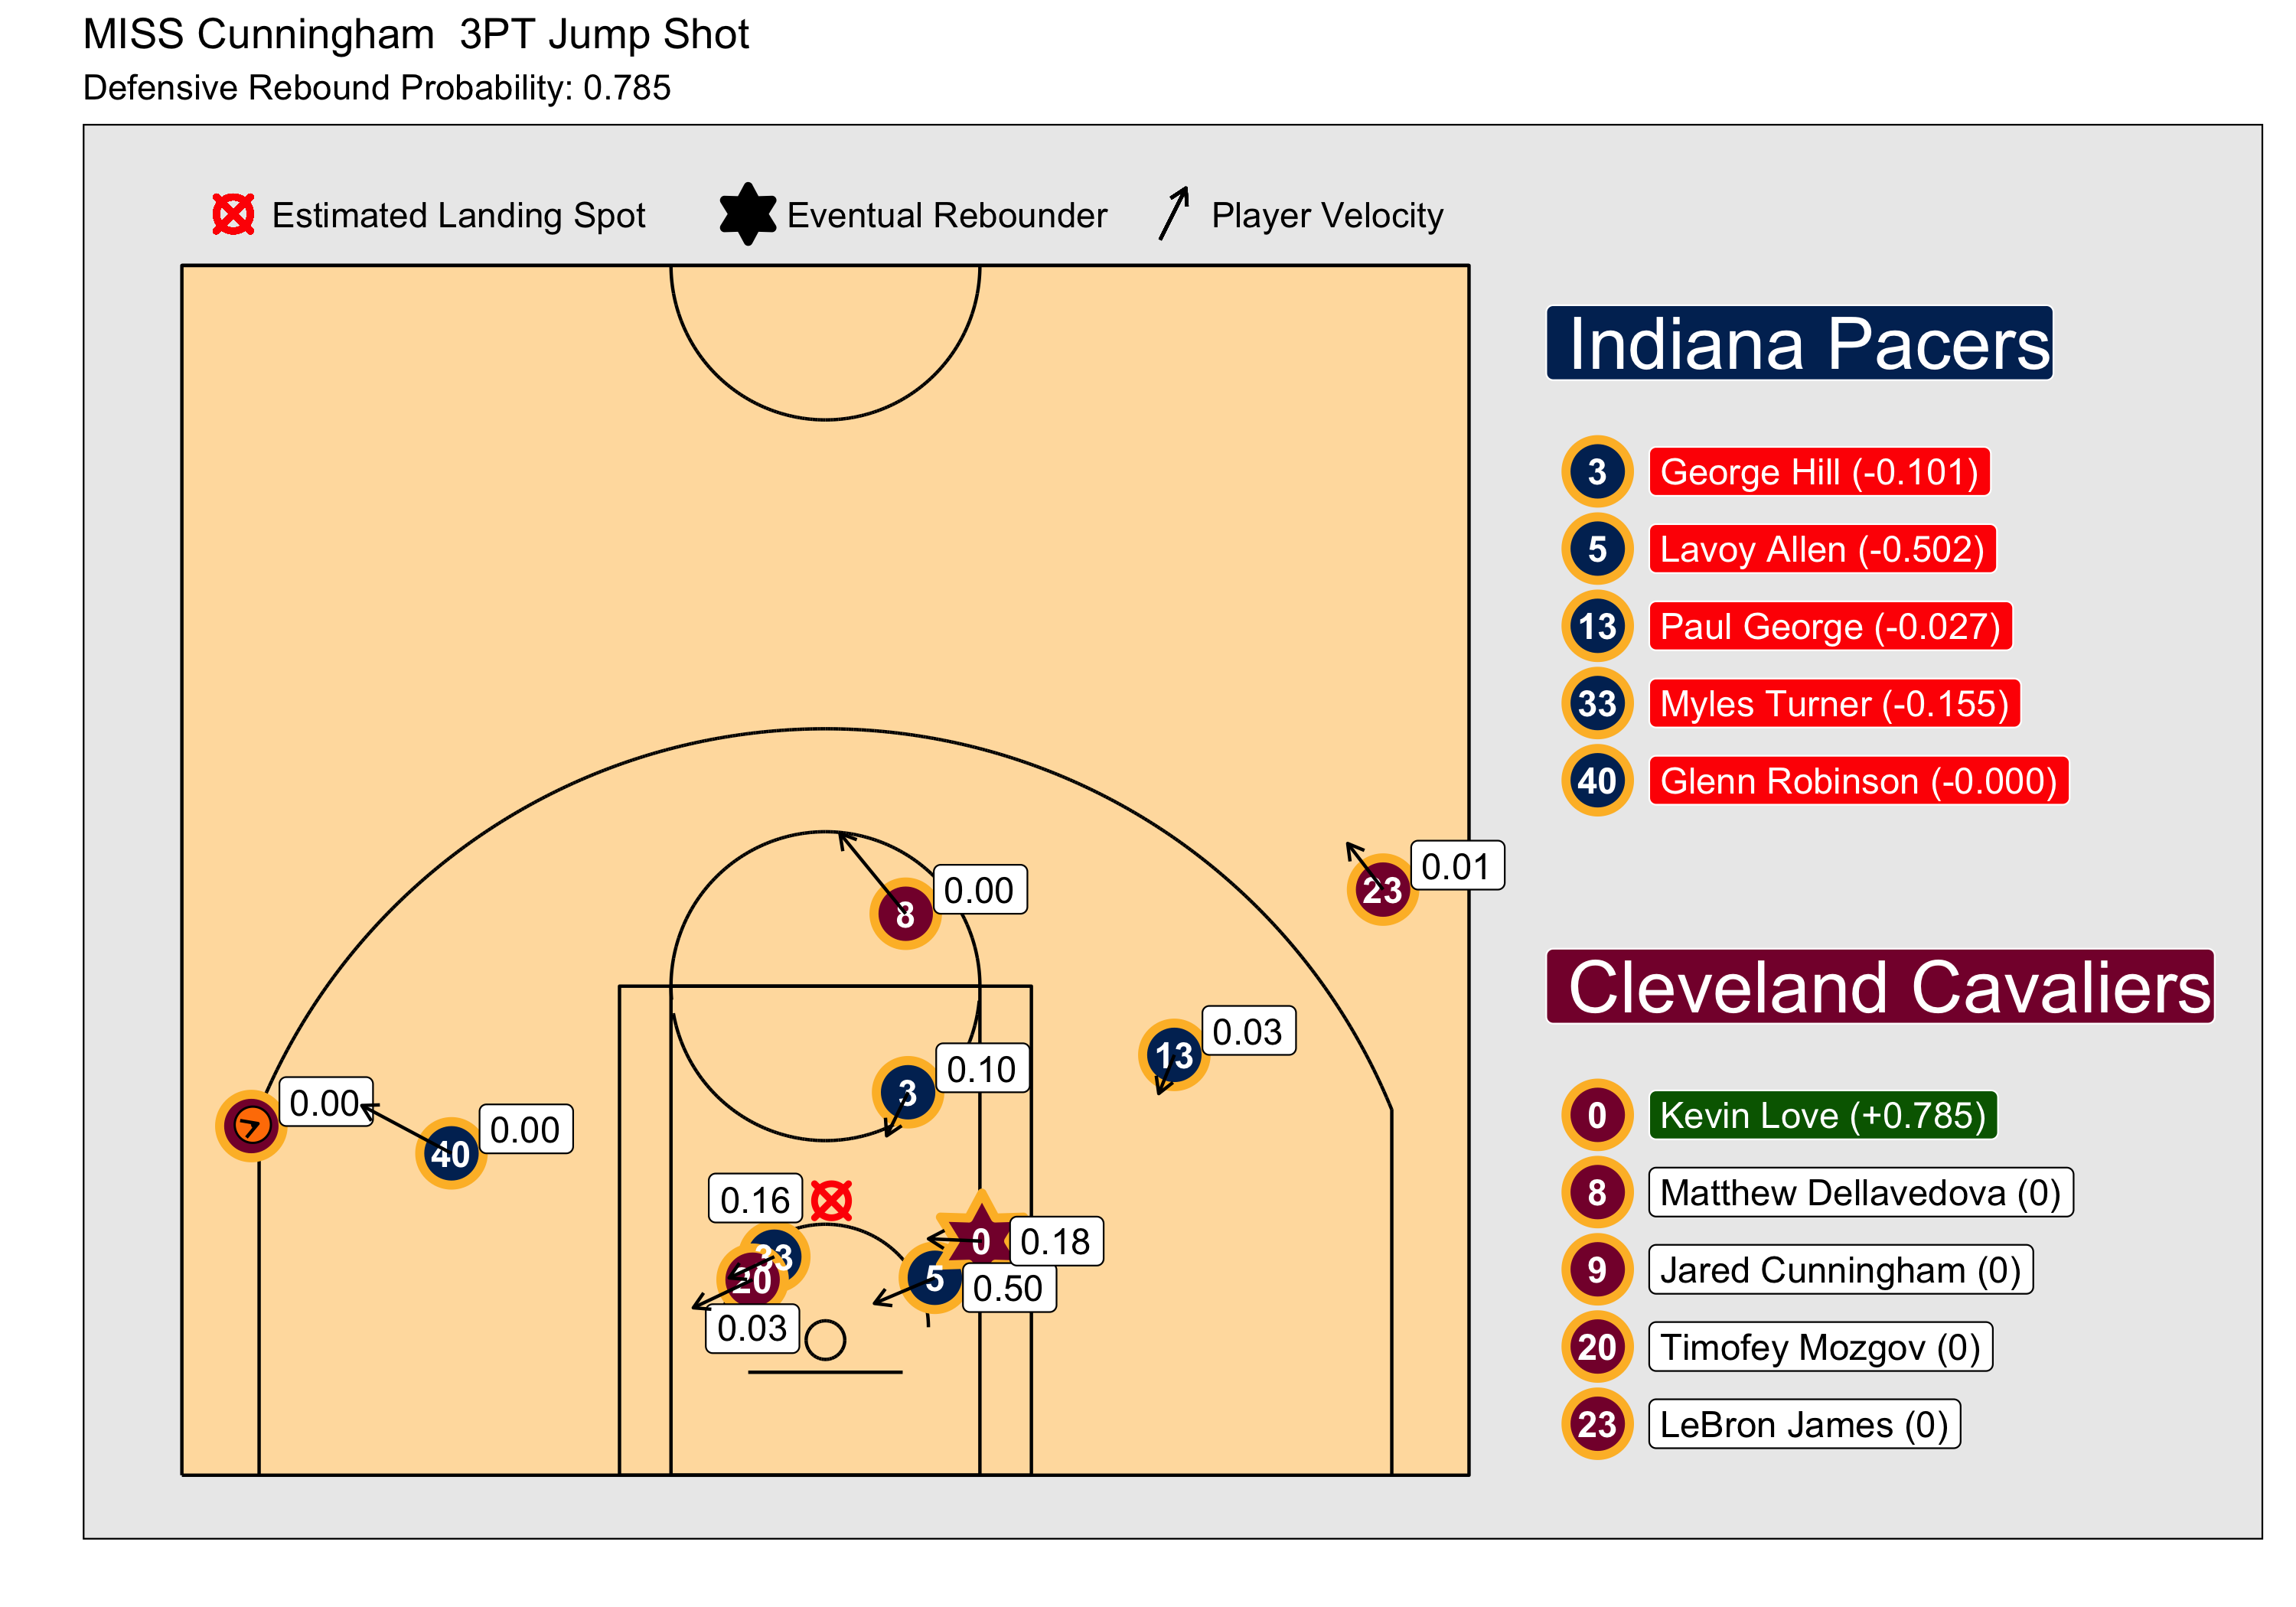
\includegraphics[width=1\columnwidth]{KLoveGoodPlayWithScores.png}
\caption{\bf{Example Play with Player Net Team Rebounds Added Values}}
\label{fig:KLoveGoodPlayWithScores}
\end{figure}

\noindent
On this play, ReboundNet predicts Lavoy Allen to be the eventual rebounder by assigning him a play high 50\% chance of recording a rebound. It assigned Kevin Love, who Lavoy Allen is boxing--out, an 18\% chance of recording a rebound. Despite this, we see that it was Kevin Love who recorded a rebound on the play. The computed $\reallywidehat{\text{NetREB}}$ values for all players, according to the above equation, are displayed next to their name on the right side of the figure. A player like Glenn Robinson, who was guarding the shooter and had slim chance of recording a rebound on the play, is barely debited any net rebounds despite his team failing to record a rebound. On the other hand, Lavoy Allen, who was in good position to record a rebound, is debited significantly.

\bigbreak
\noindent
As with the team rebounding evaluation metrics, we can aggregate the $\reallywidehat{\text{NetREB}}$ values for each player over all of their rebounding opportunities. This gives insight into which players create rebounds for their teams, and which cost their teams rebounds. \textcolor{blue}{Table} \ref{table:PlayerScores}, below, provides the 5 best and worst non--guards according to net team rebounds added for the first half of the 2015--2016 NBA season. $\reallywidehat{\text{NetREB}}^{100}$, the metric shown in \textcolor{blue}{Table} \ref{table:PlayerScores}, quantifies the number of rebounds a player adds or costs his team over 100 rebounding opportunities. Only players that are still currently in the NBA were included, and all players must have had at least 800 rebounding opportunities to qualify.

\renewcommand{\arraystretch}{1.0}
\begin{table}[htb]
  \centering
  \caption{Net Team Rebounds Added Per 100 Opportunties (Min. 800 Opportunities)}\label{table:PlayerScores}
  \begin{tabular}{cccccc}
  \toprule
 &\multicolumn{1}{c}{{\it Best}}
&
\multicolumn{4}{c}{{\it \quad \quad \quad Worst}} \\  \cmidrule(r){2-2}\cmidrule(l){5-5}
Rank & Player & $\reallywidehat{\text{NetREB}}^{100}$ & Rank & Player & $\reallywidehat{\text{NetREB}}^{100}$ \\
	\midrule
	1 & Kevin Love & {\bf \textcolor{ForestGreen}{+2.25}} & 85 & Alex Len & {\bf \textcolor{BrickRed}{--1.80}}  \\
	2 & Ian Mahinmi & {\bf \textcolor{ForestGreen}{+1.68}} &  84 & Jahlil Okafor & {\bf \textcolor{BrickRed}{--1.57}}  \\
	3 & Paul Milsap & {\bf \textcolor{ForestGreen}{+1.37}} &  83 & Cody Zeller & {\bf \textcolor{BrickRed}{--1.57}} \\
	4 & Kahwi Leonard  & {\bf \textcolor{ForestGreen}{+1.30}} & 82 & Tyson Chandler & {\bf \textcolor{BrickRed}{--1.56}} \\
	5 & Andre Drummond & {\bf \textcolor{ForestGreen}{+1.21}} & 81 & Nerlens Noel & {\bf \textcolor{BrickRed}{--1.32}} \\
\bottomrule
  \end{tabular}
\end{table}

\noindent
The main benefit to this statistic is that it leverages ReboundNet's predictions to account for a players' rebounding environments. Unlike a statistic such as rebounds per game, which intrinsically favor centers who spend most of their time around the hoop, the net team rebounds added statistic is a fair way to measure players rebounding ability. This is because players who spend more time around the hoop will be assigned higher rebound probabilities by ReboundNet, and hence will have to grab more rebounds in order to rate well. Conversely, a player who is in a less favorable rebounding environment (possibly due to playing further away from the basket or unlucky shot bounces) would not need to grab as many rebounds to rate equivalently. 
\bigbreak
\noindent
\textcolor{blue}{Figure} \ref{fig:PlayersPlot}, below, displays the relationship between our metric and the favorability of a player's rebounding environment for all qualifying players\footnote{\href{https://archive.org/web/}{WaybackMachine} was leveraged to obtain images of players as they appeared on \href{espn.com}{ESPN} as of January, 2016. That is why LeBron and Kahwi appear as Cavs and Spurs players respectively!}.

\begin{figure}[htb]
\centering
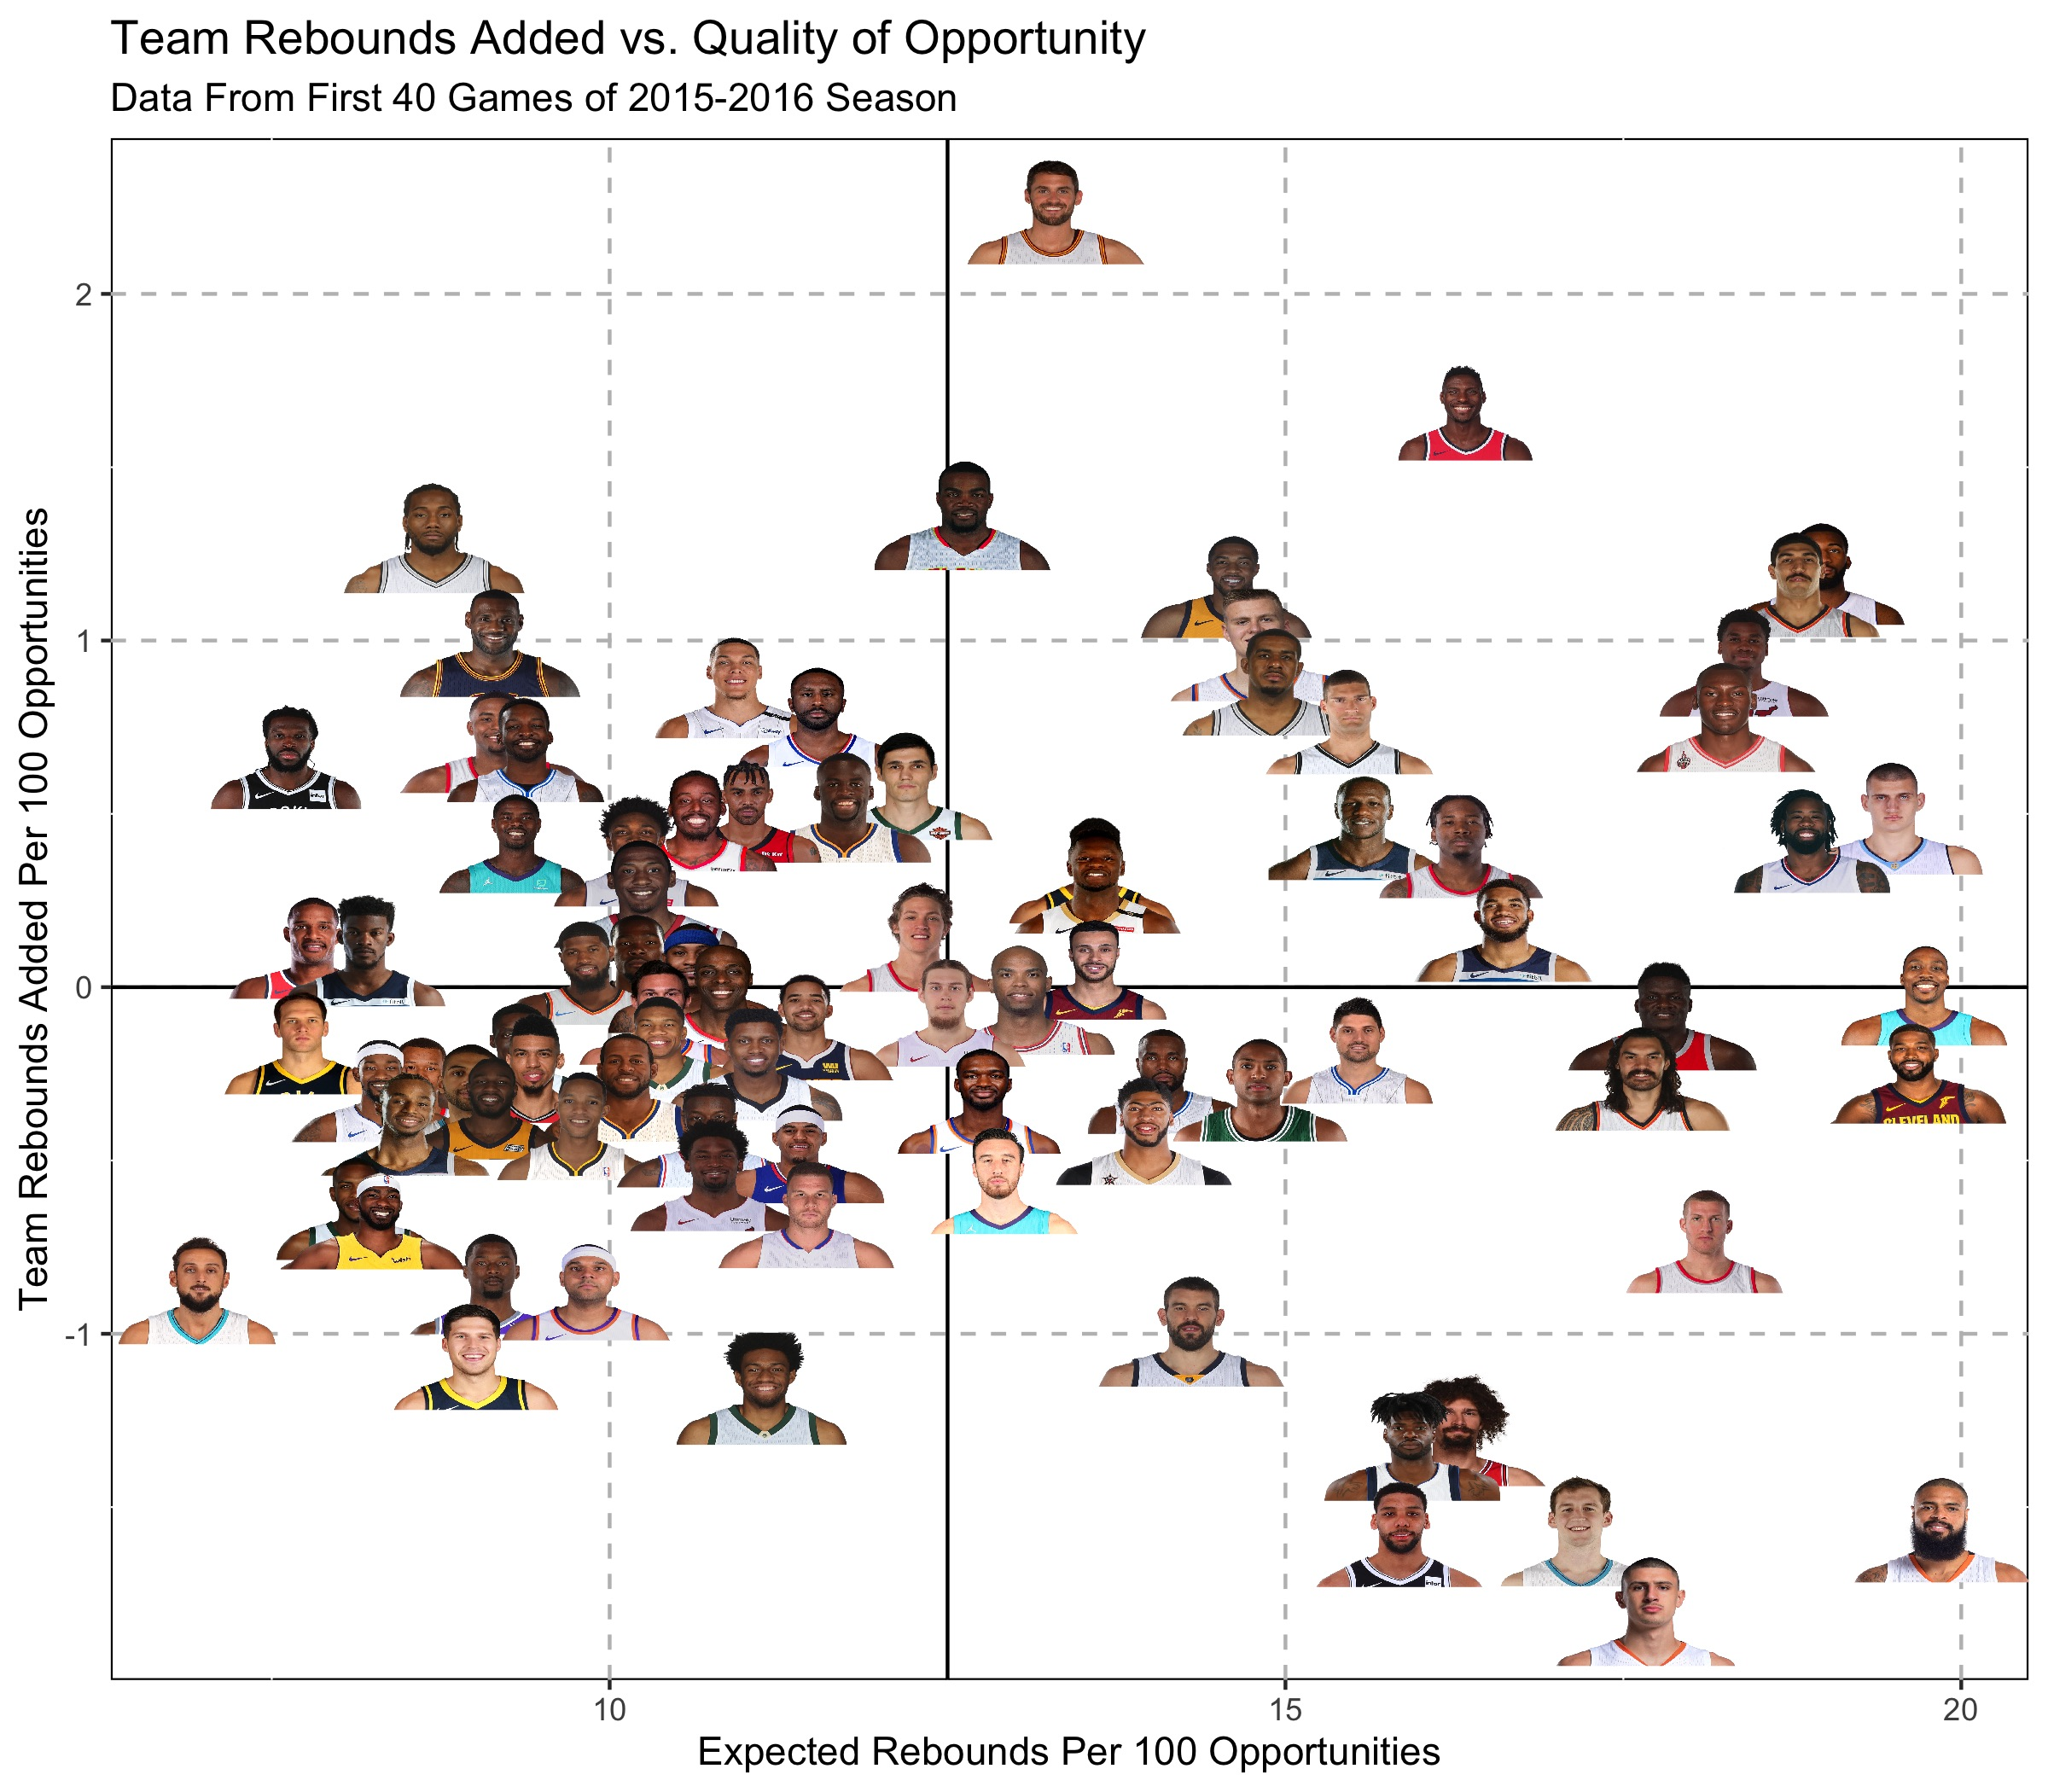
\includegraphics[width=.85\columnwidth]{PlayersPlot2.jpg}
\caption{\bf{F/C Only, Min. 800 Rebounding Opportunities}}
\label{fig:PlayersPlot}
\end{figure}

\noindent
Each player's expected rebounds over 100 possessions was computed by taking their average ReboundNet rebound probability, and multiplying by 100. Players on the far right of \textcolor{blue}{Figure} \ref{fig:PlayersPlot} (such as Andre Drummond, Dwight Howard, and Tristan Thompson) were in high rebounding environments, while players on the far left (such as Marco Belinelli, DeMarre Carroll, and LeBron James) were in low rebounding environments. Players towards the top of \textcolor{blue}{Figure} \ref{fig:PlayersPlot} added the most net team rebounds, while players at the bottom costed the most net team rebounds. With this formulation, \textcolor{blue}{Figure} \ref{fig:PlayersPlot} splits players into 4 archetypes: 

\noindent
\begin{enumerate}[labelindent = 0pt]
\itemsep0em 
\item{{\bf High--Volume Effective}: Andre Drummond, Enes Kanter, Bismack Biyombo, etc.}
\item{{\bf High--Volume Ineffective}: Alex Len, Tyson Chandler, Cody Zeller, etc.}
\item{{\bf Low--Volume Effective}: Kahwi Leonard, LeBron James, DeMarre Carrol, etc.}
\item{{\bf Low--Volume Ineffective}: Marco Belinelli, Corey Brewer, Doug McDermott, etc.}
\end{enumerate}

\noindent
Additionally, players that appear close together on our plot are similarly skilled and positioned rebounders. For example, LeBron James and Kahwi Leonard appear right next to eachother\footnote{Another interesting similarity is Julius Randle and Thad Young, where the two players are so similar that Randle almost completely covers Young.}. Similarly, players that are a far distance apart are dissimilar, such as Andre Drummond and Marco Belinelli.

\bigbreak
\noindent
It is also interesting to analyze players across different groupings. For example, \textcolor{blue}{Figure} \ref{fig:PlayersPlotCstEnv}, below, looks at a group of players in the same rebounding environment (each averages around a 9\% rebound probability per opportunity).

\begin{figure}[htb]
\centering
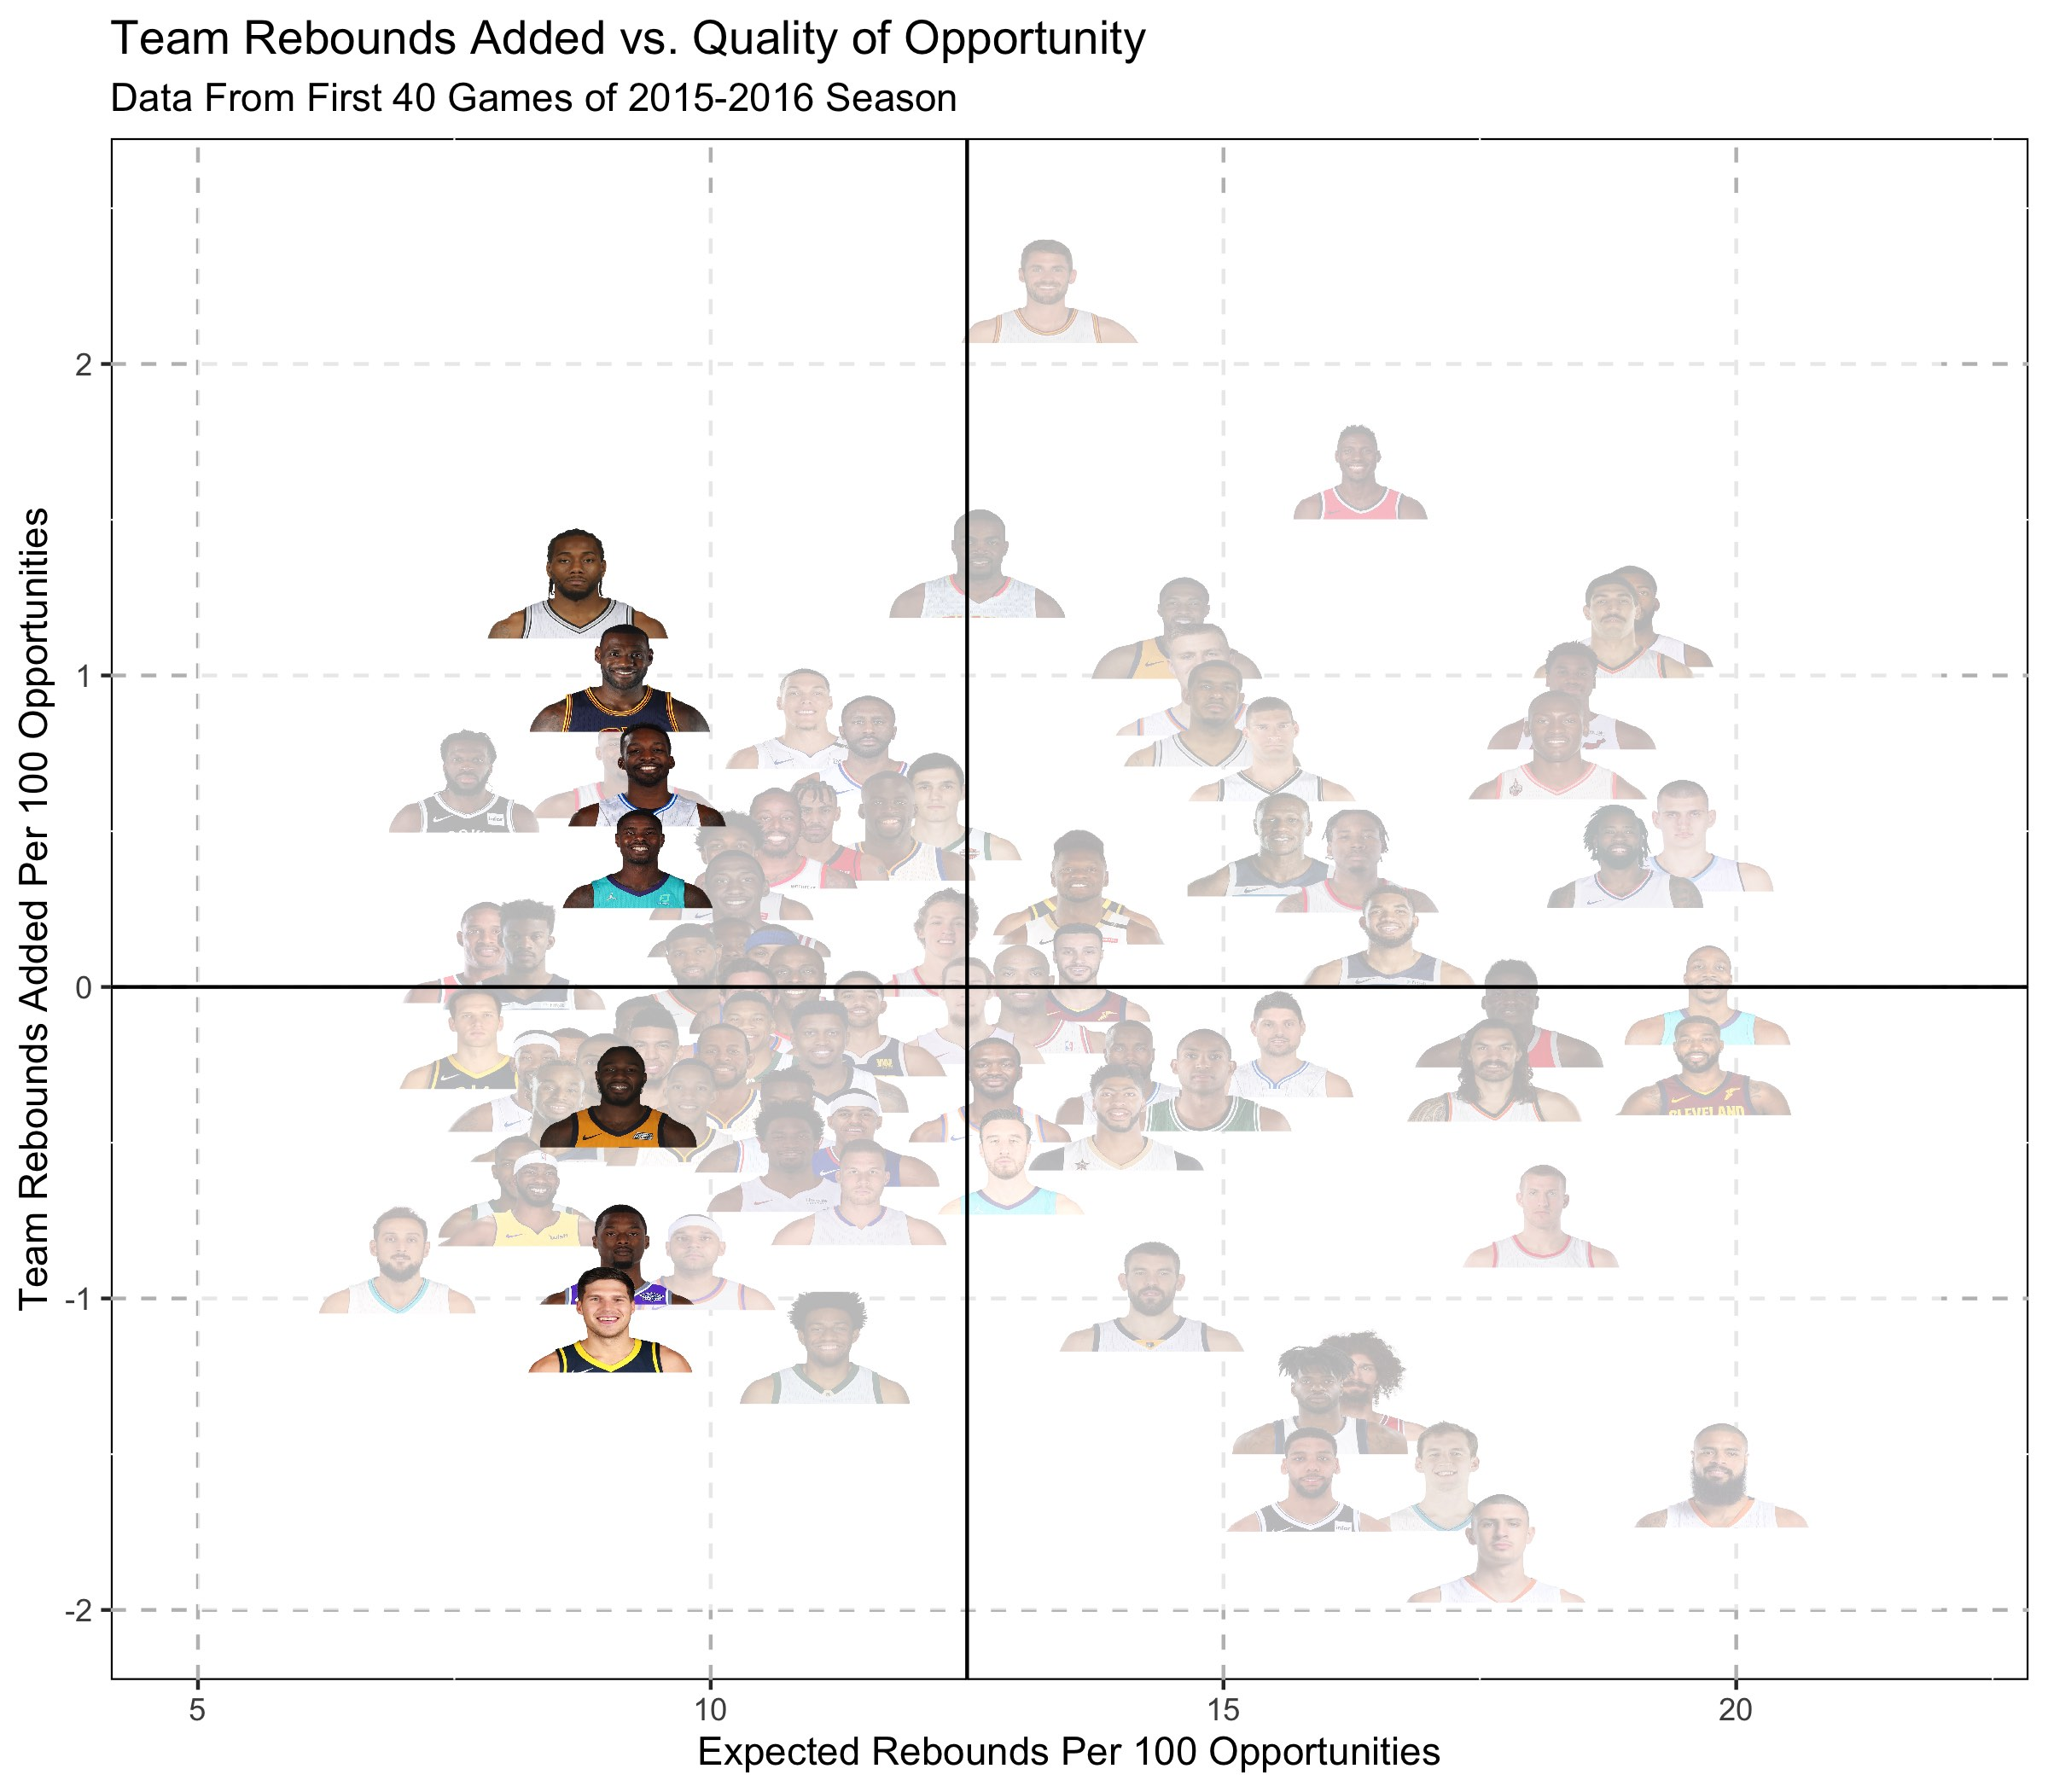
\includegraphics[width=.85\columnwidth]{PlayersPlotCstEnv2.jpg}
\caption{\bf{Group with Constant Rebounding Environment but Varying Skill}}
\label{fig:PlayersPlotCstEnv}
\end{figure}
\clearpage
\noindent
As we move from bottom to top, we go from players with the least rebounding ability (Doug McDermott) to the most ability (Kahwi Leonard) in that rebounding environment. Likewise, we could imagine moving horizontally along the plot, where we are moving along lines of constant skill, but varying the rebounding environment. It is fun to check out different groupings, and they all seem to make intuitive sense from our experience as fans.

\bigbreak
\noindent
For the curious reader, the same plot shown in \textcolor{blue}{Figure} \ref{fig:PlayersPlot}  is replicated for guards below. It follows intuition that Russell Westbrook, Rajan Rondo, and Tyler Johnson grade well, while Jamal Crawford and JJ Redick grade poorly.

\begin{figure}[htb]
\centering
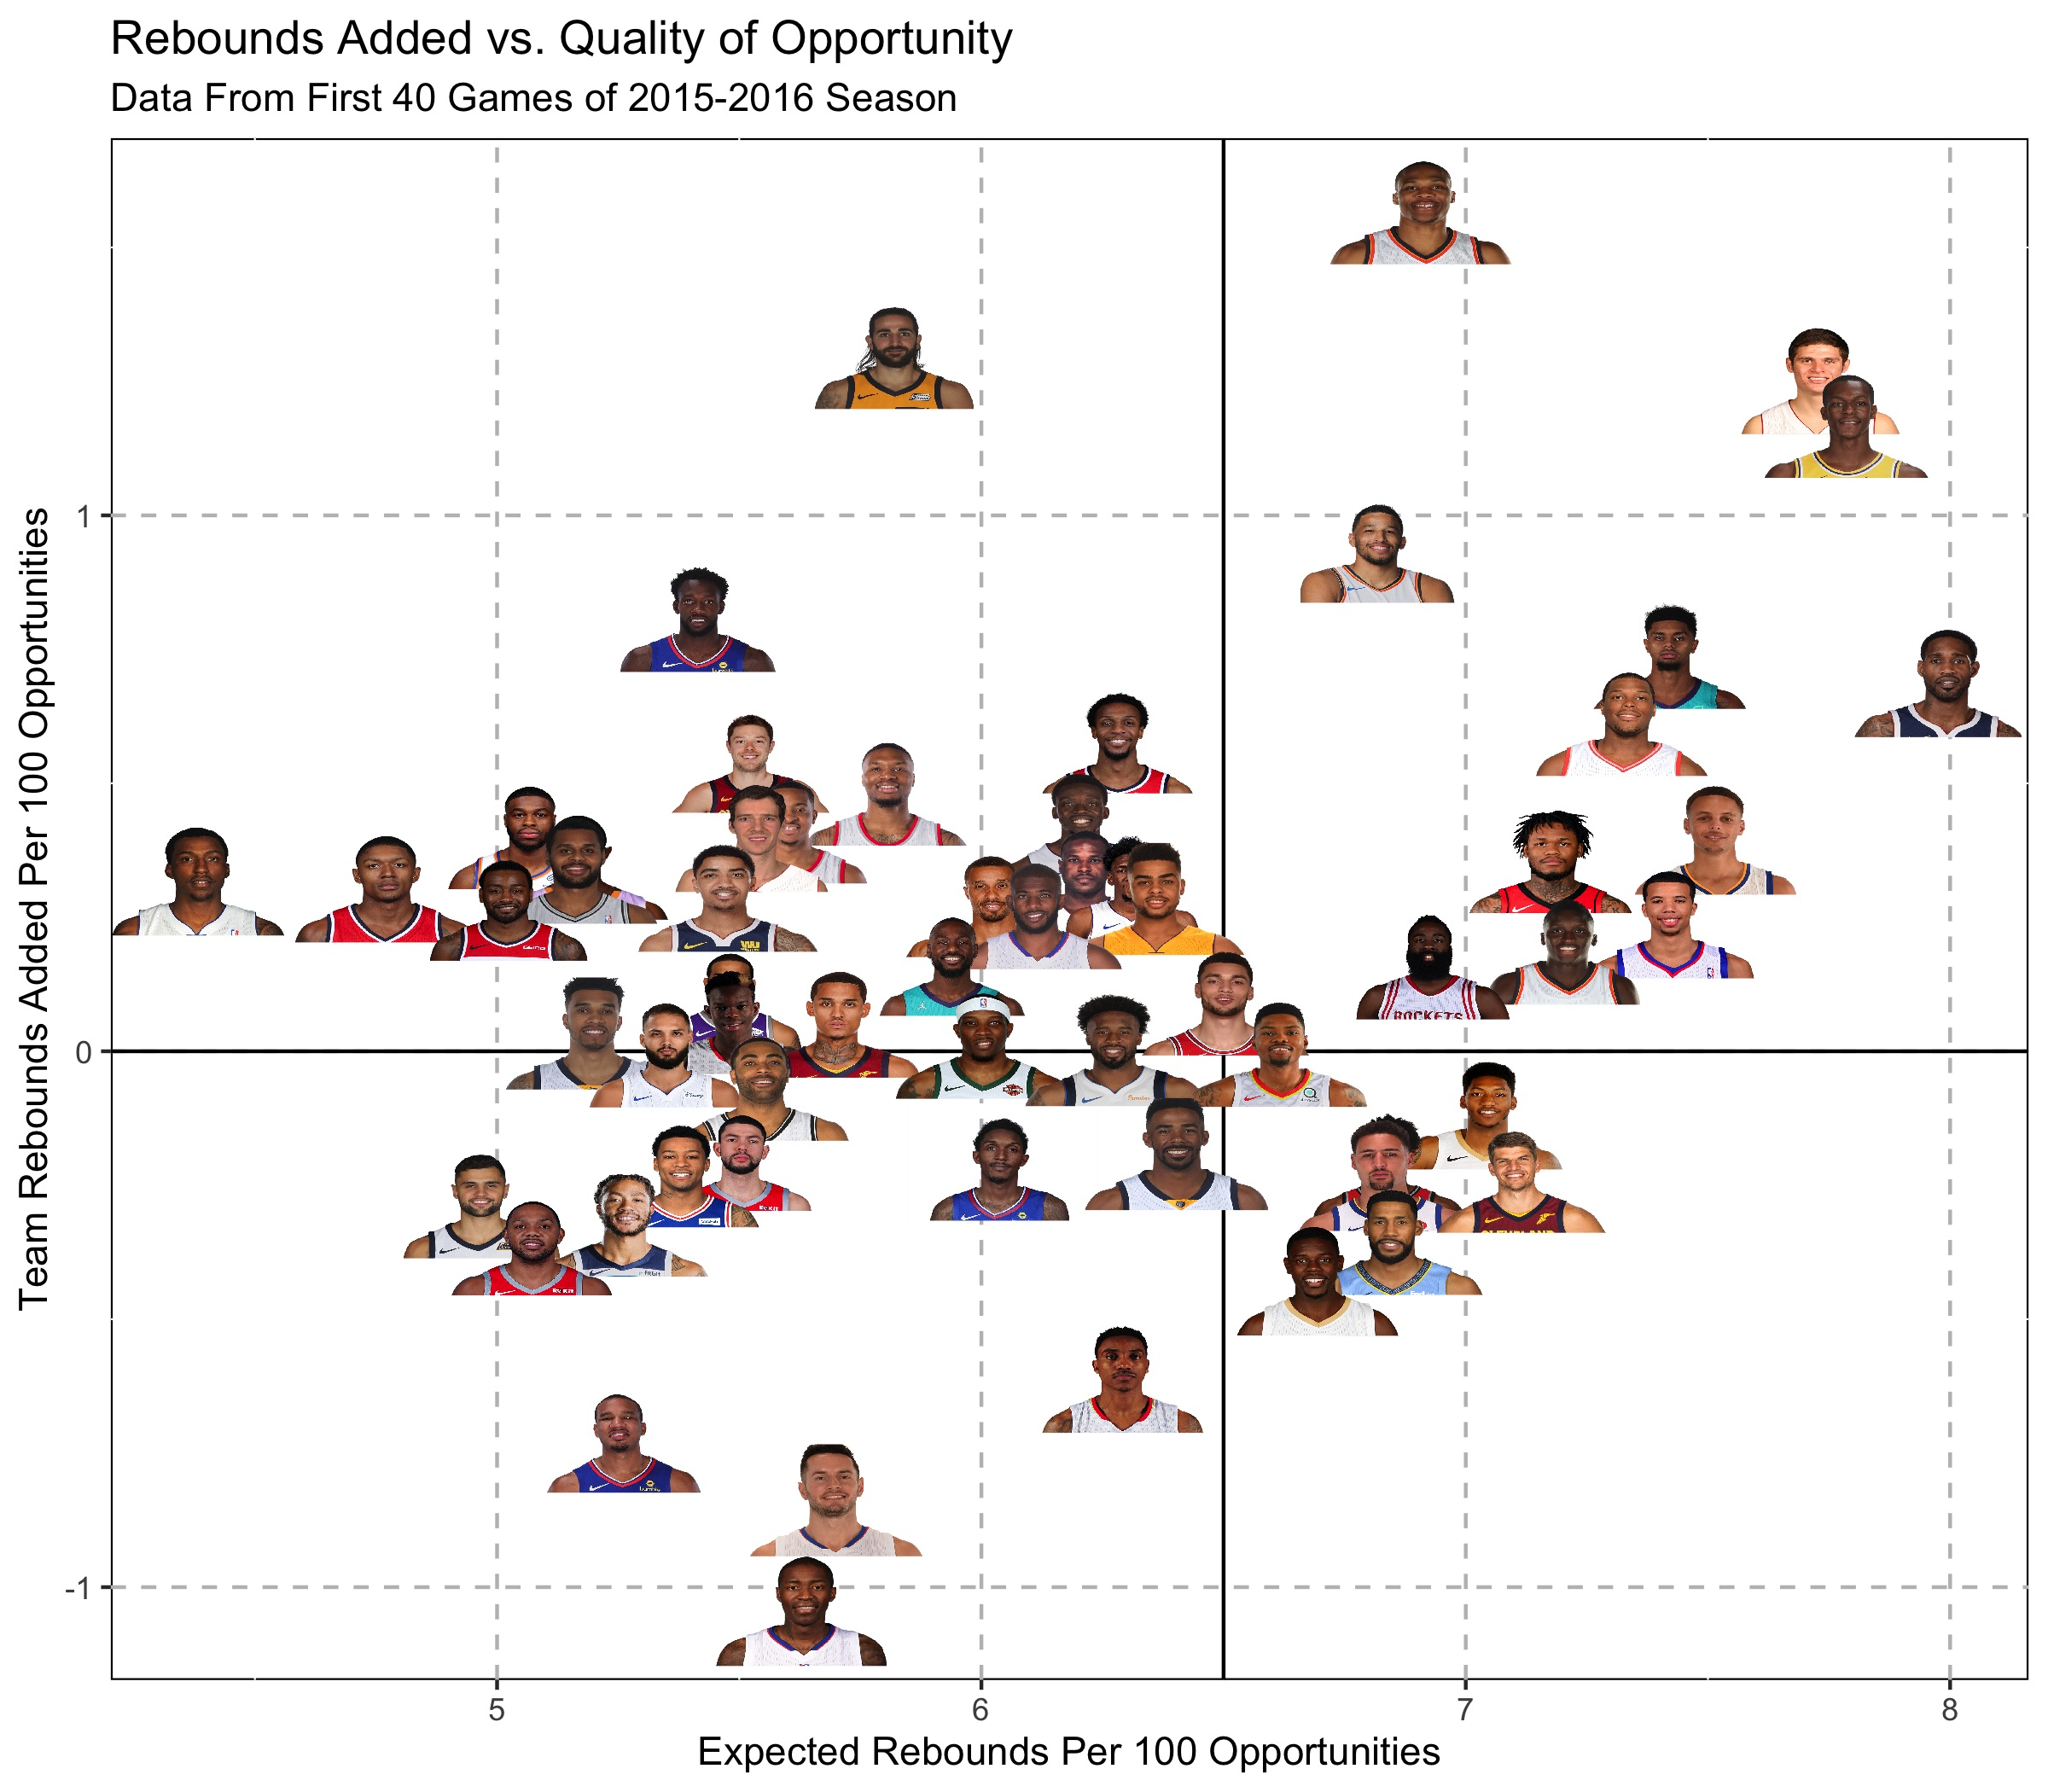
\includegraphics[width=.85\columnwidth]{GuardsPlot2.jpg}
\caption{\bf{G Only, Min. 800 Rebounding Opportunities}}
\label{fig:GuardsPlot}
\end{figure}


\end{document}
